\documentclass[twoside]{book}

% Packages required by doxygen
\usepackage{fixltx2e}
\usepackage{calc}
\usepackage{doxygen}
\usepackage[export]{adjustbox} % also loads graphicx
\usepackage{graphicx}
\usepackage[utf8]{inputenc}
\usepackage{makeidx}
\usepackage{multicol}
\usepackage{multirow}
\PassOptionsToPackage{warn}{textcomp}
\usepackage{textcomp}
\usepackage[nointegrals]{wasysym}
\usepackage[table]{xcolor}

% Font selection
\usepackage[T1]{fontenc}
\usepackage[scaled=.90]{helvet}
\usepackage{courier}
\usepackage{amssymb}
\usepackage{sectsty}
\renewcommand{\familydefault}{\sfdefault}
\allsectionsfont{%
  \fontseries{bc}\selectfont%
  \color{darkgray}%
}
\renewcommand{\DoxyLabelFont}{%
  \fontseries{bc}\selectfont%
  \color{darkgray}%
}
\newcommand{\+}{\discretionary{\mbox{\scriptsize$\hookleftarrow$}}{}{}}

% Page & text layout
\usepackage{geometry}
\geometry{%
  a4paper,%
  top=2.5cm,%
  bottom=2.5cm,%
  left=2.5cm,%
  right=2.5cm%
}
\tolerance=750
\hfuzz=15pt
\hbadness=750
\setlength{\emergencystretch}{15pt}
\setlength{\parindent}{0cm}
\setlength{\parskip}{3ex plus 2ex minus 2ex}
\makeatletter
\renewcommand{\paragraph}{%
  \@startsection{paragraph}{4}{0ex}{-1.0ex}{1.0ex}{%
    \normalfont\normalsize\bfseries\SS@parafont%
  }%
}
\renewcommand{\subparagraph}{%
  \@startsection{subparagraph}{5}{0ex}{-1.0ex}{1.0ex}{%
    \normalfont\normalsize\bfseries\SS@subparafont%
  }%
}
\makeatother

% Headers & footers
\usepackage{fancyhdr}
\pagestyle{fancyplain}
\fancyhead[LE]{\fancyplain{}{\bfseries\thepage}}
\fancyhead[CE]{\fancyplain{}{}}
\fancyhead[RE]{\fancyplain{}{\bfseries\leftmark}}
\fancyhead[LO]{\fancyplain{}{\bfseries\rightmark}}
\fancyhead[CO]{\fancyplain{}{}}
\fancyhead[RO]{\fancyplain{}{\bfseries\thepage}}
\fancyfoot[LE]{\fancyplain{}{}}
\fancyfoot[CE]{\fancyplain{}{}}
\fancyfoot[RE]{\fancyplain{}{\bfseries\scriptsize Generated by Doxygen }}
\fancyfoot[LO]{\fancyplain{}{\bfseries\scriptsize Generated by Doxygen }}
\fancyfoot[CO]{\fancyplain{}{}}
\fancyfoot[RO]{\fancyplain{}{}}
\renewcommand{\footrulewidth}{0.4pt}
\renewcommand{\chaptermark}[1]{%
  \markboth{#1}{}%
}
\renewcommand{\sectionmark}[1]{%
  \markright{\thesection\ #1}%
}

% Indices & bibliography
\usepackage{natbib}
\usepackage[titles]{tocloft}
\setcounter{tocdepth}{3}
\setcounter{secnumdepth}{5}
\makeindex

% Hyperlinks (required, but should be loaded last)
\usepackage{ifpdf}
\ifpdf
  \usepackage[pdftex,pagebackref=true]{hyperref}
\else
  \usepackage[ps2pdf,pagebackref=true]{hyperref}
\fi
\hypersetup{%
  colorlinks=true,%
  linkcolor=blue,%
  citecolor=blue,%
  unicode%
}

% Custom commands
\newcommand{\clearemptydoublepage}{%
  \newpage{\pagestyle{empty}\cleardoublepage}%
}

\usepackage{caption}
\captionsetup{labelsep=space,justification=centering,font={bf},singlelinecheck=off,skip=4pt,position=top}

%===== C O N T E N T S =====

\begin{document}

% Titlepage & ToC
\hypersetup{pageanchor=false,
             bookmarksnumbered=true,
             pdfencoding=unicode
            }
\pagenumbering{roman}
\begin{titlepage}
\vspace*{7cm}
\begin{center}%
{\Large Caixa Preta }\\
\vspace*{1cm}
{\large Generated by Doxygen 1.8.11}\\
\end{center}
\end{titlepage}
\clearemptydoublepage
\tableofcontents
\clearemptydoublepage
\pagenumbering{arabic}
\hypersetup{pageanchor=true}

%--- Begin generated contents ---
\chapter{Hierarchical Index}
\section{Class Hierarchy}
This inheritance list is sorted roughly, but not completely, alphabetically\+:\begin{DoxyCompactList}
\item \contentsline{section}{Button}{\pageref{class_button}}{}
\item \contentsline{section}{E\+E\+P\+R\+OM}{\pageref{class_e_e_p_r_o_m}}{}
\item \contentsline{section}{Firmware}{\pageref{class_firmware}}{}
\item \contentsline{section}{G\+P\+Sdata}{\pageref{struct_g_p_sdata}}{}
\item \contentsline{section}{L\+CD}{\pageref{class_l_c_d}}{}
\item \contentsline{section}{Leds}{\pageref{class_leds}}{}
\item \contentsline{section}{M\+PU}{\pageref{class_m_p_u}}{}
\item \contentsline{section}{Raw\+Degrees}{\pageref{struct_raw_degrees}}{}
\item \contentsline{section}{S\+PI}{\pageref{class_s_p_i}}{}
\item \contentsline{section}{S\+R\+AM}{\pageref{class_s_r_a_m}}{}
\item \contentsline{section}{Timer5}{\pageref{class_timer5}}{}
\item \contentsline{section}{Tiny\+G\+P\+S\+Custom}{\pageref{class_tiny_g_p_s_custom}}{}
\item \contentsline{section}{Tiny\+G\+P\+S\+Date}{\pageref{struct_tiny_g_p_s_date}}{}
\item \contentsline{section}{Tiny\+G\+P\+S\+Decimal}{\pageref{struct_tiny_g_p_s_decimal}}{}
\begin{DoxyCompactList}
\item \contentsline{section}{Tiny\+G\+P\+S\+Altitude}{\pageref{struct_tiny_g_p_s_altitude}}{}
\item \contentsline{section}{Tiny\+G\+P\+S\+Course}{\pageref{struct_tiny_g_p_s_course}}{}
\item \contentsline{section}{Tiny\+G\+P\+S\+H\+D\+OP}{\pageref{struct_tiny_g_p_s_h_d_o_p}}{}
\item \contentsline{section}{Tiny\+G\+P\+S\+Speed}{\pageref{struct_tiny_g_p_s_speed}}{}
\end{DoxyCompactList}
\item \contentsline{section}{Tiny\+G\+P\+S\+Integer}{\pageref{struct_tiny_g_p_s_integer}}{}
\item \contentsline{section}{Tiny\+G\+P\+S\+Location}{\pageref{struct_tiny_g_p_s_location}}{}
\item \contentsline{section}{Tiny\+G\+P\+S\+Plus}{\pageref{class_tiny_g_p_s_plus}}{}
\item \contentsline{section}{Tiny\+G\+P\+S\+Time}{\pageref{struct_tiny_g_p_s_time}}{}
\item \contentsline{section}{T\+WI}{\pageref{class_t_w_i}}{}
\item \contentsline{section}{U\+S\+A\+RT}{\pageref{class_u_s_a_r_t}}{}
\end{DoxyCompactList}

\chapter{Class Index}
\section{Class List}
Here are the classes, structs, unions and interfaces with brief descriptions\+:\begin{DoxyCompactList}
\item\contentsline{section}{{\bf Button} }{\pageref{class_button}}{}
\item\contentsline{section}{{\bf E\+E\+P\+R\+OM} }{\pageref{class_e_e_p_r_o_m}}{}
\item\contentsline{section}{{\bf Firmware} }{\pageref{class_firmware}}{}
\item\contentsline{section}{{\bf G\+P\+Sdata} }{\pageref{struct_g_p_sdata}}{}
\item\contentsline{section}{{\bf L\+CD} }{\pageref{class_l_c_d}}{}
\item\contentsline{section}{{\bf Leds} }{\pageref{class_leds}}{}
\item\contentsline{section}{{\bf M\+PU} }{\pageref{class_m_p_u}}{}
\item\contentsline{section}{{\bf Raw\+Degrees} }{\pageref{struct_raw_degrees}}{}
\item\contentsline{section}{{\bf S\+PI} }{\pageref{class_s_p_i}}{}
\item\contentsline{section}{{\bf S\+R\+AM} }{\pageref{class_s_r_a_m}}{}
\item\contentsline{section}{{\bf Timer5} }{\pageref{class_timer5}}{}
\item\contentsline{section}{{\bf Tiny\+G\+P\+S\+Altitude} }{\pageref{struct_tiny_g_p_s_altitude}}{}
\item\contentsline{section}{{\bf Tiny\+G\+P\+S\+Course} }{\pageref{struct_tiny_g_p_s_course}}{}
\item\contentsline{section}{{\bf Tiny\+G\+P\+S\+Custom} }{\pageref{class_tiny_g_p_s_custom}}{}
\item\contentsline{section}{{\bf Tiny\+G\+P\+S\+Date} }{\pageref{struct_tiny_g_p_s_date}}{}
\item\contentsline{section}{{\bf Tiny\+G\+P\+S\+Decimal} }{\pageref{struct_tiny_g_p_s_decimal}}{}
\item\contentsline{section}{{\bf Tiny\+G\+P\+S\+H\+D\+OP} }{\pageref{struct_tiny_g_p_s_h_d_o_p}}{}
\item\contentsline{section}{{\bf Tiny\+G\+P\+S\+Integer} }{\pageref{struct_tiny_g_p_s_integer}}{}
\item\contentsline{section}{{\bf Tiny\+G\+P\+S\+Location} }{\pageref{struct_tiny_g_p_s_location}}{}
\item\contentsline{section}{{\bf Tiny\+G\+P\+S\+Plus} }{\pageref{class_tiny_g_p_s_plus}}{}
\item\contentsline{section}{{\bf Tiny\+G\+P\+S\+Speed} }{\pageref{struct_tiny_g_p_s_speed}}{}
\item\contentsline{section}{{\bf Tiny\+G\+P\+S\+Time} }{\pageref{struct_tiny_g_p_s_time}}{}
\item\contentsline{section}{{\bf T\+WI} }{\pageref{class_t_w_i}}{}
\item\contentsline{section}{{\bf U\+S\+A\+RT} }{\pageref{class_u_s_a_r_t}}{}
\end{DoxyCompactList}

\chapter{Class Documentation}
\hypertarget{class_button}{}\section{Button Class Reference}
\label{class_button}\index{Button@{Button}}
\subsection*{Public Member Functions}
\begin{DoxyCompactItemize}
\item 
\hyperlink{class_button_a3b36df1ae23c58aedb9e15a713159459}{Button} ()
\item 
void \hyperlink{class_button_a01a47c09c53b9fd4b635e337aebf76be}{read\+Buttons} ()
\item 
bool \hyperlink{class_button_ac0663845722d920a837d5fbd38b794df}{read\+Buffer} (char $\ast$key)
\end{DoxyCompactItemize}


\subsection{Constructor \& Destructor Documentation}
\index{Button@{Button}!Button@{Button}}
\index{Button@{Button}!Button@{Button}}
\subsubsection[{\texorpdfstring{Button()}{Button()}}]{\setlength{\rightskip}{0pt plus 5cm}Button\+::\+Button (
\begin{DoxyParamCaption}
{}
\end{DoxyParamCaption}
)}\hypertarget{class_button_a3b36df1ae23c58aedb9e15a713159459}{}\label{class_button_a3b36df1ae23c58aedb9e15a713159459}
Construtor da classe. Inicializa os botões. 

\subsection{Member Function Documentation}
\index{Button@{Button}!read\+Buffer@{read\+Buffer}}
\index{read\+Buffer@{read\+Buffer}!Button@{Button}}
\subsubsection[{\texorpdfstring{read\+Buffer(char $\ast$key)}{readBuffer(char *key)}}]{\setlength{\rightskip}{0pt plus 5cm}bool Button\+::read\+Buffer (
\begin{DoxyParamCaption}
\item[{char $\ast$}]{key}
\end{DoxyParamCaption}
)}\hypertarget{class_button_ac0663845722d920a837d5fbd38b794df}{}\label{class_button_ac0663845722d920a837d5fbd38b794df}
Tira uma chave do buffer e retorna se houve sucesso 
\begin{DoxyParams}{Parameters}
{\em key} & ponteiro para a variável que vai receber o valor da chave acionada \\
\hline
\end{DoxyParams}
\begin{DoxyReturn}{Returns}
T\+R\+UE se havia chave no buffer e F\+A\+L\+SE se não havia chave no buffer 
\end{DoxyReturn}
\index{Button@{Button}!read\+Buttons@{read\+Buttons}}
\index{read\+Buttons@{read\+Buttons}!Button@{Button}}
\subsubsection[{\texorpdfstring{read\+Buttons()}{readButtons()}}]{\setlength{\rightskip}{0pt plus 5cm}void Button\+::read\+Buttons (
\begin{DoxyParamCaption}
{}
\end{DoxyParamCaption}
)}\hypertarget{class_button_a01a47c09c53b9fd4b635e337aebf76be}{}\label{class_button_a01a47c09c53b9fd4b635e337aebf76be}
Lê as chaves e coloca no buffer. Monitora as chaves em 20 Hz 

The documentation for this class was generated from the following file\+:\begin{DoxyCompactItemize}
\item 
headers/Button.\+h\end{DoxyCompactItemize}

\section{L\+CD Class Reference}
\label{class_l_c_d}\index{L\+CD@{L\+CD}}
\subsection*{Public Member Functions}
\begin{DoxyCompactItemize}
\item 
{\bf L\+CD} ()
\item 
void {\bf start\+Config} ()
\item 
void {\bf caracter} (byte code, byte $\ast$vet)
\item 
void {\bf print\+Dec16} (word nr, byte lin, byte col)
\item 
void {\bf print\+Dec8} (byte nr, byte lin, byte col)
\item 
void {\bf print\+Hex16} (word nr, byte lin, byte col)
\item 
void {\bf print\+Hex8} (byte nr, byte lin, byte col)
\item 
void {\bf print\+Char8} (byte nr, byte lin, byte col)
\item 
void {\bf load\+Buffer} (byte $\ast$vet, byte lin, byte col)
\item 
void {\bf load\+L\+CD} (byte lin, byte coli, byte colf)
\item 
void {\bf load\+Buffer\+White} ()
\item 
void {\bf cursor} (byte on)
\item 
void {\bf command} (byte dado)
\item 
void {\bf print\+Char} (byte dado)
\item 
void {\bf set\+Cursor} (byte pos)
\item 
byte {\bf read\+Address\+Counter} ()
\item 
bool {\bf is\+Busy} ()
\item 
void {\bf back\+Light} (bool on)
\end{DoxyCompactItemize}
\subsection*{Public Attributes}
\begin{DoxyCompactItemize}
\item 
byte {\bf lcd\+\_\+buffer} [4][20]
\item 
volatile bool {\bf lcd\+\_\+flag0}
\item 
volatile bool {\bf lcd\+\_\+flag1}
\end{DoxyCompactItemize}


\subsection{Constructor \& Destructor Documentation}
\index{L\+CD@{L\+CD}!L\+CD@{L\+CD}}
\index{L\+CD@{L\+CD}!L\+CD@{L\+CD}}
\subsubsection[{L\+C\+D()}]{\setlength{\rightskip}{0pt plus 5cm}L\+C\+D\+::\+L\+CD (
\begin{DoxyParamCaption}
{}
\end{DoxyParamCaption}
)}\label{class_l_c_d_a00bb2db1390721abc7b24ac4b8c276c8}
Construtor da classe. Inicia os pinos. 

\subsection{Member Function Documentation}
\index{L\+CD@{L\+CD}!back\+Light@{back\+Light}}
\index{back\+Light@{back\+Light}!L\+CD@{L\+CD}}
\subsubsection[{back\+Light(bool on)}]{\setlength{\rightskip}{0pt plus 5cm}void L\+C\+D\+::back\+Light (
\begin{DoxyParamCaption}
\item[{bool}]{on}
\end{DoxyParamCaption}
)}\label{class_l_c_d_a3342a83c4cc8afa0da7c0ea8ef10d549}
Acende e apaga o Back Light 
\begin{DoxyParams}{Parameters}
{\em on} & T\+R\+UE para ligar o back light e F\+A\+L\+SE para desligar o back light \\
\hline
\end{DoxyParams}
\index{L\+CD@{L\+CD}!caracter@{caracter}}
\index{caracter@{caracter}!L\+CD@{L\+CD}}
\subsubsection[{caracter(byte code, byte $\ast$vet)}]{\setlength{\rightskip}{0pt plus 5cm}void L\+C\+D\+::caracter (
\begin{DoxyParamCaption}
\item[{byte}]{code, }
\item[{byte $\ast$}]{vet}
\end{DoxyParamCaption}
)}\label{class_l_c_d_a9868c6740864f198778e24b1f38147b9}
Cria um caracterer especial 
\begin{DoxyParams}{Parameters}
{\em code} & código do caracter \\
\hline
{\em vet} & vetor de 8 posições com o mapa de pontos \\
\hline
\end{DoxyParams}
\index{L\+CD@{L\+CD}!command@{command}}
\index{command@{command}!L\+CD@{L\+CD}}
\subsubsection[{command(byte dado)}]{\setlength{\rightskip}{0pt plus 5cm}void L\+C\+D\+::command (
\begin{DoxyParamCaption}
\item[{byte}]{dado}
\end{DoxyParamCaption}
)}\label{class_l_c_d_a9be7dae5cf36e971cf40472fddb3a2bc}
Escrever um comando (instrução) no \doxyref{L\+CD}{p.}{class_l_c_d} 
\begin{DoxyParams}{Parameters}
{\em dado} & instrução \\
\hline
\end{DoxyParams}
\index{L\+CD@{L\+CD}!cursor@{cursor}}
\index{cursor@{cursor}!L\+CD@{L\+CD}}
\subsubsection[{cursor(byte on)}]{\setlength{\rightskip}{0pt plus 5cm}void L\+C\+D\+::cursor (
\begin{DoxyParamCaption}
\item[{byte}]{on}
\end{DoxyParamCaption}
)}\label{class_l_c_d_ae42ed5491b5e32a2e740d57aebe4e8dd}
Liga e desliga o cursor piscante 
\begin{DoxyParams}{Parameters}
{\em on} & ON para ligar o cursor e O\+FF para desligar o cursor \\
\hline
\end{DoxyParams}
\index{L\+CD@{L\+CD}!is\+Busy@{is\+Busy}}
\index{is\+Busy@{is\+Busy}!L\+CD@{L\+CD}}
\subsubsection[{is\+Busy()}]{\setlength{\rightskip}{0pt plus 5cm}bool L\+C\+D\+::is\+Busy (
\begin{DoxyParamCaption}
{}
\end{DoxyParamCaption}
)}\label{class_l_c_d_a9a83a13b931a2ccbb17c80a119869d24}
Verifica se o \doxyref{L\+CD}{p.}{class_l_c_d} está ocupado \begin{DoxyReturn}{Returns}
T\+R\+UE se tiver ocupado e F\+A\+L\+SE se estiver livre 
\end{DoxyReturn}
\index{L\+CD@{L\+CD}!load\+Buffer@{load\+Buffer}}
\index{load\+Buffer@{load\+Buffer}!L\+CD@{L\+CD}}
\subsubsection[{load\+Buffer(byte $\ast$vet, byte lin, byte col)}]{\setlength{\rightskip}{0pt plus 5cm}void L\+C\+D\+::load\+Buffer (
\begin{DoxyParamCaption}
\item[{byte $\ast$}]{vet, }
\item[{byte}]{lin, }
\item[{byte}]{col}
\end{DoxyParamCaption}
)}\label{class_l_c_d_a47a75e256bcc0f76cdd75e5c425e2bf6}
Trasferir uma string para o lcd\+\_\+buffer. Transfere até encontrar o \char`\"{}\textbackslash{}0\char`\"{} 
\begin{DoxyParams}{Parameters}
{\em vet} & ponteiro para string \\
\hline
{\em lin} & linha de início \\
\hline
{\em col} & coluna de início \\
\hline
\end{DoxyParams}
\index{L\+CD@{L\+CD}!load\+Buffer\+White@{load\+Buffer\+White}}
\index{load\+Buffer\+White@{load\+Buffer\+White}!L\+CD@{L\+CD}}
\subsubsection[{load\+Buffer\+White()}]{\setlength{\rightskip}{0pt plus 5cm}void L\+C\+D\+::load\+Buffer\+White (
\begin{DoxyParamCaption}
{}
\end{DoxyParamCaption}
)}\label{class_l_c_d_a70a46c817aa34b2a91c153a3dd0e9591}
Colocar branco (0x20) em todo o buffer do \doxyref{L\+CD}{p.}{class_l_c_d} \index{L\+CD@{L\+CD}!load\+L\+CD@{load\+L\+CD}}
\index{load\+L\+CD@{load\+L\+CD}!L\+CD@{L\+CD}}
\subsubsection[{load\+L\+C\+D(byte lin, byte coli, byte colf)}]{\setlength{\rightskip}{0pt plus 5cm}void L\+C\+D\+::load\+L\+CD (
\begin{DoxyParamCaption}
\item[{byte}]{lin, }
\item[{byte}]{coli, }
\item[{byte}]{colf}
\end{DoxyParamCaption}
)}\label{class_l_c_d_a3ec14c7f40b08492f65779cbd662e3d1}
Trasferir do lcd\+\_\+buffer para o \doxyref{L\+CD}{p.}{class_l_c_d}. Só transfere uma linha 
\begin{DoxyParams}{Parameters}
{\em lin} & linha de início \\
\hline
{\em coli} & coluna de início \\
\hline
{\em colf} & coluna final (inclusa) \\
\hline
\end{DoxyParams}
\index{L\+CD@{L\+CD}!print\+Char@{print\+Char}}
\index{print\+Char@{print\+Char}!L\+CD@{L\+CD}}
\subsubsection[{print\+Char(byte dado)}]{\setlength{\rightskip}{0pt plus 5cm}void L\+C\+D\+::print\+Char (
\begin{DoxyParamCaption}
\item[{byte}]{dado}
\end{DoxyParamCaption}
)}\label{class_l_c_d_a02c39e2c9424ef4c5ec8a4d83c59b6e6}
Escrever uma caracter no \doxyref{L\+CD}{p.}{class_l_c_d} 
\begin{DoxyParams}{Parameters}
{\em dado} & caracter \\
\hline
\end{DoxyParams}
\index{L\+CD@{L\+CD}!print\+Char8@{print\+Char8}}
\index{print\+Char8@{print\+Char8}!L\+CD@{L\+CD}}
\subsubsection[{print\+Char8(byte nr, byte lin, byte col)}]{\setlength{\rightskip}{0pt plus 5cm}void L\+C\+D\+::print\+Char8 (
\begin{DoxyParamCaption}
\item[{byte}]{nr, }
\item[{byte}]{lin, }
\item[{byte}]{col}
\end{DoxyParamCaption}
)}\label{class_l_c_d_aed5147061cc9761230e2977a5de9fa5d}
Imprime uma letra em 8 bits 
\begin{DoxyParams}{Parameters}
{\em nr} & char \\
\hline
{\em lin} & linha de início \\
\hline
{\em col} & coluna de início \\
\hline
\end{DoxyParams}
\index{L\+CD@{L\+CD}!print\+Dec16@{print\+Dec16}}
\index{print\+Dec16@{print\+Dec16}!L\+CD@{L\+CD}}
\subsubsection[{print\+Dec16(word nr, byte lin, byte col)}]{\setlength{\rightskip}{0pt plus 5cm}void L\+C\+D\+::print\+Dec16 (
\begin{DoxyParamCaption}
\item[{word}]{nr, }
\item[{byte}]{lin, }
\item[{byte}]{col}
\end{DoxyParamCaption}
)}\label{class_l_c_d_a368ef1f6a659bb7a28b4dabc3ed66c93}
Imprime um decimal de 16 bits 
\begin{DoxyParams}{Parameters}
{\em nr} & número \\
\hline
{\em lin} & linha de início \\
\hline
{\em col} & coluna de início \\
\hline
\end{DoxyParams}
\index{L\+CD@{L\+CD}!print\+Dec8@{print\+Dec8}}
\index{print\+Dec8@{print\+Dec8}!L\+CD@{L\+CD}}
\subsubsection[{print\+Dec8(byte nr, byte lin, byte col)}]{\setlength{\rightskip}{0pt plus 5cm}void L\+C\+D\+::print\+Dec8 (
\begin{DoxyParamCaption}
\item[{byte}]{nr, }
\item[{byte}]{lin, }
\item[{byte}]{col}
\end{DoxyParamCaption}
)}\label{class_l_c_d_a9081bd4c9f6e1cfe1aa855a2005eb101}
Imprime um decimal de 8 bits 
\begin{DoxyParams}{Parameters}
{\em nr} & número \\
\hline
{\em lin} & linha de início \\
\hline
{\em col} & coluna de início \\
\hline
\end{DoxyParams}
\index{L\+CD@{L\+CD}!print\+Hex16@{print\+Hex16}}
\index{print\+Hex16@{print\+Hex16}!L\+CD@{L\+CD}}
\subsubsection[{print\+Hex16(word nr, byte lin, byte col)}]{\setlength{\rightskip}{0pt plus 5cm}void L\+C\+D\+::print\+Hex16 (
\begin{DoxyParamCaption}
\item[{word}]{nr, }
\item[{byte}]{lin, }
\item[{byte}]{col}
\end{DoxyParamCaption}
)}\label{class_l_c_d_a66ca9248294d9ed3ac3db52c2389da7a}
Imprime um hexadecimal de 16 bits 
\begin{DoxyParams}{Parameters}
{\em nr} & número \\
\hline
{\em lin} & linha de início \\
\hline
{\em col} & coluna de início \\
\hline
\end{DoxyParams}
\index{L\+CD@{L\+CD}!print\+Hex8@{print\+Hex8}}
\index{print\+Hex8@{print\+Hex8}!L\+CD@{L\+CD}}
\subsubsection[{print\+Hex8(byte nr, byte lin, byte col)}]{\setlength{\rightskip}{0pt plus 5cm}void L\+C\+D\+::print\+Hex8 (
\begin{DoxyParamCaption}
\item[{byte}]{nr, }
\item[{byte}]{lin, }
\item[{byte}]{col}
\end{DoxyParamCaption}
)}\label{class_l_c_d_a088b602412fafc11266296b8537edc1f}
Imprime um hexadecimal de 8 bits 
\begin{DoxyParams}{Parameters}
{\em nr} & número \\
\hline
{\em lin} & linha de início \\
\hline
{\em col} & coluna de início \\
\hline
\end{DoxyParams}
\index{L\+CD@{L\+CD}!read\+Address\+Counter@{read\+Address\+Counter}}
\index{read\+Address\+Counter@{read\+Address\+Counter}!L\+CD@{L\+CD}}
\subsubsection[{read\+Address\+Counter()}]{\setlength{\rightskip}{0pt plus 5cm}byte L\+C\+D\+::read\+Address\+Counter (
\begin{DoxyParamCaption}
{}
\end{DoxyParamCaption}
)}\label{class_l_c_d_a9285bcefcb08e96f0aaf7cad56a5b4e0}
Ler contador de endereços \begin{DoxyReturn}{Returns}
Contador de endereços 
\end{DoxyReturn}
\index{L\+CD@{L\+CD}!set\+Cursor@{set\+Cursor}}
\index{set\+Cursor@{set\+Cursor}!L\+CD@{L\+CD}}
\subsubsection[{set\+Cursor(byte pos)}]{\setlength{\rightskip}{0pt plus 5cm}void L\+C\+D\+::set\+Cursor (
\begin{DoxyParamCaption}
\item[{byte}]{pos}
\end{DoxyParamCaption}
)}\label{class_l_c_d_a124c2100ce0dded2a83f586fe618eee3}
Posicionar o cursor 
\begin{DoxyParams}{Parameters}
{\em pos} & posição \\
\hline
\end{DoxyParams}
\index{L\+CD@{L\+CD}!start\+Config@{start\+Config}}
\index{start\+Config@{start\+Config}!L\+CD@{L\+CD}}
\subsubsection[{start\+Config()}]{\setlength{\rightskip}{0pt plus 5cm}void L\+C\+D\+::start\+Config (
\begin{DoxyParamCaption}
{}
\end{DoxyParamCaption}
)}\label{class_l_c_d_abb7937561b3bc75fd672003b81e388f7}
Configura o \doxyref{L\+CD}{p.}{class_l_c_d} para começar o uso 

\subsection{Member Data Documentation}
\index{L\+CD@{L\+CD}!lcd\+\_\+buffer@{lcd\+\_\+buffer}}
\index{lcd\+\_\+buffer@{lcd\+\_\+buffer}!L\+CD@{L\+CD}}
\subsubsection[{lcd\+\_\+buffer}]{\setlength{\rightskip}{0pt plus 5cm}byte L\+C\+D\+::lcd\+\_\+buffer[4][20]}\label{class_l_c_d_a5768e304cd832c5ac495c805f1ef7de9}
Buffer para o \doxyref{L\+CD}{p.}{class_l_c_d} [lin][col] terminar cada linha com Zero \index{L\+CD@{L\+CD}!lcd\+\_\+flag0@{lcd\+\_\+flag0}}
\index{lcd\+\_\+flag0@{lcd\+\_\+flag0}!L\+CD@{L\+CD}}
\subsubsection[{lcd\+\_\+flag0}]{\setlength{\rightskip}{0pt plus 5cm}volatile bool L\+C\+D\+::lcd\+\_\+flag0}\label{class_l_c_d_ab8dc463b096981437ced6749c072b06c}
Flag para indicar que a linha 0 deve atualizar \index{L\+CD@{L\+CD}!lcd\+\_\+flag1@{lcd\+\_\+flag1}}
\index{lcd\+\_\+flag1@{lcd\+\_\+flag1}!L\+CD@{L\+CD}}
\subsubsection[{lcd\+\_\+flag1}]{\setlength{\rightskip}{0pt plus 5cm}volatile bool L\+C\+D\+::lcd\+\_\+flag1}\label{class_l_c_d_adc6d0cdd4dcb57a392daadbda71562de}
Flag para indicar que a linha 1 deve atualizar 

The documentation for this class was generated from the following file\+:\begin{DoxyCompactItemize}
\item 
headers/L\+C\+D.\+h\end{DoxyCompactItemize}

\hypertarget{class_leds}{}\section{Leds Class Reference}
\label{class_leds}\index{Leds@{Leds}}
\subsection*{Public Member Functions}
\begin{DoxyCompactItemize}
\item 
\hyperlink{class_leds_a240103486293e11969e1260e96fd6801}{Leds} ()
\item 
void \hyperlink{class_leds_aae0a51182e5cbf41b066f1931b528e3b}{green} (byte on)
\item 
void \hyperlink{class_leds_a1e638204035fdde890dda92b1d371954}{yellow} (byte on)
\item 
void \hyperlink{class_leds_a8da7ba5d99a1943c9e0709930ad551df}{red} (byte on)
\item 
void \hyperlink{class_leds_abe056fe9a1c82d84cf52c9b557ea6430}{turn\+Off\+All} ()
\item 
void \hyperlink{class_leds_a0f785e583bff2cf5c9f1196594d94b59}{turn\+On\+All} ()
\end{DoxyCompactItemize}


\subsection{Constructor \& Destructor Documentation}
\index{Leds@{Leds}!Leds@{Leds}}
\index{Leds@{Leds}!Leds@{Leds}}
\subsubsection[{\texorpdfstring{Leds()}{Leds()}}]{\setlength{\rightskip}{0pt plus 5cm}Leds\+::\+Leds (
\begin{DoxyParamCaption}
{}
\end{DoxyParamCaption}
)}\hypertarget{class_leds_a240103486293e11969e1260e96fd6801}{}\label{class_leds_a240103486293e11969e1260e96fd6801}
Construtor da classe. Inicia as portas dos \hyperlink{class_leds}{Leds} como saída e os desliga. 

\subsection{Member Function Documentation}
\index{Leds@{Leds}!green@{green}}
\index{green@{green}!Leds@{Leds}}
\subsubsection[{\texorpdfstring{green(byte on)}{green(byte on)}}]{\setlength{\rightskip}{0pt plus 5cm}void Leds\+::green (
\begin{DoxyParamCaption}
\item[{byte}]{on}
\end{DoxyParamCaption}
)}\hypertarget{class_leds_aae0a51182e5cbf41b066f1931b528e3b}{}\label{class_leds_aae0a51182e5cbf41b066f1931b528e3b}
Liga, desliga ou troca o estado do led verde 
\begin{DoxyParams}{Parameters}
{\em on} & ON para ligar, O\+FF para desligar e T\+O\+G\+G\+LE para trocar o estado \\
\hline
\end{DoxyParams}
\index{Leds@{Leds}!red@{red}}
\index{red@{red}!Leds@{Leds}}
\subsubsection[{\texorpdfstring{red(byte on)}{red(byte on)}}]{\setlength{\rightskip}{0pt plus 5cm}void Leds\+::red (
\begin{DoxyParamCaption}
\item[{byte}]{on}
\end{DoxyParamCaption}
)}\hypertarget{class_leds_a8da7ba5d99a1943c9e0709930ad551df}{}\label{class_leds_a8da7ba5d99a1943c9e0709930ad551df}
Liga, desliga ou troca o estado do led vermelho 
\begin{DoxyParams}{Parameters}
{\em on} & ON para ligar, O\+FF para desligar e T\+O\+G\+G\+LE para trocar o estado \\
\hline
\end{DoxyParams}
\index{Leds@{Leds}!turn\+Off\+All@{turn\+Off\+All}}
\index{turn\+Off\+All@{turn\+Off\+All}!Leds@{Leds}}
\subsubsection[{\texorpdfstring{turn\+Off\+All()}{turnOffAll()}}]{\setlength{\rightskip}{0pt plus 5cm}void Leds\+::turn\+Off\+All (
\begin{DoxyParamCaption}
{}
\end{DoxyParamCaption}
)}\hypertarget{class_leds_abe056fe9a1c82d84cf52c9b557ea6430}{}\label{class_leds_abe056fe9a1c82d84cf52c9b557ea6430}
Desliga todos os leds \index{Leds@{Leds}!turn\+On\+All@{turn\+On\+All}}
\index{turn\+On\+All@{turn\+On\+All}!Leds@{Leds}}
\subsubsection[{\texorpdfstring{turn\+On\+All()}{turnOnAll()}}]{\setlength{\rightskip}{0pt plus 5cm}void Leds\+::turn\+On\+All (
\begin{DoxyParamCaption}
{}
\end{DoxyParamCaption}
)}\hypertarget{class_leds_a0f785e583bff2cf5c9f1196594d94b59}{}\label{class_leds_a0f785e583bff2cf5c9f1196594d94b59}
Liga todos os leds \index{Leds@{Leds}!yellow@{yellow}}
\index{yellow@{yellow}!Leds@{Leds}}
\subsubsection[{\texorpdfstring{yellow(byte on)}{yellow(byte on)}}]{\setlength{\rightskip}{0pt plus 5cm}void Leds\+::yellow (
\begin{DoxyParamCaption}
\item[{byte}]{on}
\end{DoxyParamCaption}
)}\hypertarget{class_leds_a1e638204035fdde890dda92b1d371954}{}\label{class_leds_a1e638204035fdde890dda92b1d371954}
Liga, desliga ou troca o estado do led amarelo 
\begin{DoxyParams}{Parameters}
{\em on} & ON para ligar, O\+FF para desligar e T\+O\+G\+G\+LE para trocar o estado \\
\hline
\end{DoxyParams}


The documentation for this class was generated from the following file\+:\begin{DoxyCompactItemize}
\item 
headers/Leds.\+h\end{DoxyCompactItemize}

\hypertarget{class_m_p_u}{}\section{M\+PU Class Reference}
\label{class_m_p_u}\index{M\+PU@{M\+PU}}
\subsection*{Public Member Functions}
\begin{DoxyCompactItemize}
\item 
\hyperlink{class_m_p_u_a0deec2f8e8170b2e21ee015940d550b6}{M\+PU} ()
\item 
\hyperlink{class_m_p_u_a524c777097cbc9ae0c3942d1d115787c}{M\+PU} (int freq)
\item 
bool \hyperlink{class_m_p_u_a048d708b54073a32c0daa6b1b8e4a365}{write\+Register} (byte reg, byte dado)
\item 
byte \hyperlink{class_m_p_u_aa42e2711c058fa9abe5af418ae4cf647}{read\+Register} (byte reg)
\item 
bool \hyperlink{class_m_p_u_a691201f2735fc1d9270166e0cb190e79}{write\+Block\+Data} (byte reg, byte $\ast$dado, byte qtd)
\item 
void \hyperlink{class_m_p_u_abbb1b779a2a248020210dddf074c077a}{read\+Block\+Data} (byte reg, byte $\ast$dado, byte qtd)
\item 
byte \hyperlink{class_m_p_u_a37db9ff5d63c1bccd5a9a5d08ae58fe7}{who\+AmI} ()
\item 
void \hyperlink{class_m_p_u_a1ccf05ed209b8305bf6a74a7daffb880}{wake\+Up} ()
\item 
void \hyperlink{class_m_p_u_a93abaf43da55d96c26ef4212afc671f9}{sleep} ()
\item 
void \hyperlink{class_m_p_u_ac4cc325b1514c121892ed86f292dad99}{set\+Scale} (byte gfs, byte afs)
\item 
void \hyperlink{class_m_p_u_a0240f4cd1c4ba1528ac86eccb9da261a}{read\+Average\+Accel\+Temp\+Gyros} (word rpt)
\item 
void \hyperlink{class_m_p_u_ad0d6f8dfbf2e0b86f4918deaa1e1e8ff}{read\+Accel\+Temp\+Gyros} ()
\item 
bool \hyperlink{class_m_p_u_a5559e8a86d055d7e6e9f19ff65851fae}{self\+Test} ()
\item 
void \hyperlink{class_m_p_u_a9978b29c17eee830126686e082799808}{calibrate} (int16\+\_\+t $\ast$bias, float $\ast$valor)
\end{DoxyCompactItemize}
\subsection*{Public Attributes}
\begin{DoxyCompactItemize}
\item 
int \hyperlink{class_m_p_u_a970d6ef662d744e848058828d4f20de6}{axi}
\item 
int \hyperlink{class_m_p_u_a84628559828dd5476ee2a8888d26d2a7}{ayi}
\item 
int \hyperlink{class_m_p_u_a8307625db324101f2c1c0db433253b63}{azi}
\item 
int \hyperlink{class_m_p_u_ab953ed7e9b1ef0b70f0ad97e137616c5}{tpi}
\item 
int \hyperlink{class_m_p_u_a16a4ca3ef12197ee9876e71033c20f4f}{gxi}
\item 
int \hyperlink{class_m_p_u_a5ae8eb6cc6be2a2a91957a34d59dc468}{gyi}
\item 
int \hyperlink{class_m_p_u_ac43952f01d98aad441ff08f53aa281a8}{gzi}
\end{DoxyCompactItemize}


\subsection{Constructor \& Destructor Documentation}
\index{M\+PU@{M\+PU}!M\+PU@{M\+PU}}
\index{M\+PU@{M\+PU}!M\+PU@{M\+PU}}
\subsubsection[{\texorpdfstring{M\+P\+U()}{MPU()}}]{\setlength{\rightskip}{0pt plus 5cm}M\+P\+U\+::\+M\+PU (
\begin{DoxyParamCaption}
{}
\end{DoxyParamCaption}
)}\hypertarget{class_m_p_u_a0deec2f8e8170b2e21ee015940d550b6}{}\label{class_m_p_u_a0deec2f8e8170b2e21ee015940d550b6}
Construtor default da classe. \index{M\+PU@{M\+PU}!M\+PU@{M\+PU}}
\index{M\+PU@{M\+PU}!M\+PU@{M\+PU}}
\subsubsection[{\texorpdfstring{M\+P\+U(int freq)}{MPU(int freq)}}]{\setlength{\rightskip}{0pt plus 5cm}M\+P\+U\+::\+M\+PU (
\begin{DoxyParamCaption}
\item[{int}]{freq}
\end{DoxyParamCaption}
)}\hypertarget{class_m_p_u_a524c777097cbc9ae0c3942d1d115787c}{}\label{class_m_p_u_a524c777097cbc9ae0c3942d1d115787c}
Construtor da classe. Coloca o \hyperlink{class_m_p_u}{M\+PU} num estado conhecido. Algumas operações podem ser redundantes. 
\begin{DoxyParams}{Parameters}
{\em freq} & frequência utilizada \\
\hline
\end{DoxyParams}


\subsection{Member Function Documentation}
\index{M\+PU@{M\+PU}!calibrate@{calibrate}}
\index{calibrate@{calibrate}!M\+PU@{M\+PU}}
\subsubsection[{\texorpdfstring{calibrate(int16\+\_\+t $\ast$bias, float $\ast$valor)}{calibrate(int16_t *bias, float *valor)}}]{\setlength{\rightskip}{0pt plus 5cm}void M\+P\+U\+::calibrate (
\begin{DoxyParamCaption}
\item[{int16\+\_\+t $\ast$}]{bias, }
\item[{float $\ast$}]{valor}
\end{DoxyParamCaption}
)}\hypertarget{class_m_p_u_a9978b29c17eee830126686e082799808}{}\label{class_m_p_u_a9978b29c17eee830126686e082799808}
Calibra o acelerômetro e o giroscópio do \hyperlink{class_m_p_u}{M\+PU} 
\begin{DoxyParams}{Parameters}
{\em bias} & \\
\hline
{\em valor} & \\
\hline
\end{DoxyParams}
\index{M\+PU@{M\+PU}!read\+Accel\+Temp\+Gyros@{read\+Accel\+Temp\+Gyros}}
\index{read\+Accel\+Temp\+Gyros@{read\+Accel\+Temp\+Gyros}!M\+PU@{M\+PU}}
\subsubsection[{\texorpdfstring{read\+Accel\+Temp\+Gyros()}{readAccelTempGyros()}}]{\setlength{\rightskip}{0pt plus 5cm}void M\+P\+U\+::read\+Accel\+Temp\+Gyros (
\begin{DoxyParamCaption}
{}
\end{DoxyParamCaption}
)}\hypertarget{class_m_p_u_ad0d6f8dfbf2e0b86f4918deaa1e1e8ff}{}\label{class_m_p_u_ad0d6f8dfbf2e0b86f4918deaa1e1e8ff}
Lê a aceleração, temperatura e giroscópio \index{M\+PU@{M\+PU}!read\+Average\+Accel\+Temp\+Gyros@{read\+Average\+Accel\+Temp\+Gyros}}
\index{read\+Average\+Accel\+Temp\+Gyros@{read\+Average\+Accel\+Temp\+Gyros}!M\+PU@{M\+PU}}
\subsubsection[{\texorpdfstring{read\+Average\+Accel\+Temp\+Gyros(word rpt)}{readAverageAccelTempGyros(word rpt)}}]{\setlength{\rightskip}{0pt plus 5cm}void M\+P\+U\+::read\+Average\+Accel\+Temp\+Gyros (
\begin{DoxyParamCaption}
\item[{word}]{rpt}
\end{DoxyParamCaption}
)}\hypertarget{class_m_p_u_a0240f4cd1c4ba1528ac86eccb9da261a}{}\label{class_m_p_u_a0240f4cd1c4ba1528ac86eccb9da261a}
Lê a média da aceleração, temperatura e giroscópio 
\begin{DoxyParams}{Parameters}
{\em rpt} & número de leituras que vai ser tirada a média \\
\hline
\end{DoxyParams}
\index{M\+PU@{M\+PU}!read\+Block\+Data@{read\+Block\+Data}}
\index{read\+Block\+Data@{read\+Block\+Data}!M\+PU@{M\+PU}}
\subsubsection[{\texorpdfstring{read\+Block\+Data(byte reg, byte $\ast$dado, byte qtd)}{readBlockData(byte reg, byte *dado, byte qtd)}}]{\setlength{\rightskip}{0pt plus 5cm}void M\+P\+U\+::read\+Block\+Data (
\begin{DoxyParamCaption}
\item[{byte}]{reg, }
\item[{byte $\ast$}]{dado, }
\item[{byte}]{qtd}
\end{DoxyParamCaption}
)}\hypertarget{class_m_p_u_abbb1b779a2a248020210dddf074c077a}{}\label{class_m_p_u_abbb1b779a2a248020210dddf074c077a}
Lê um bloco de dados no \hyperlink{class_m_p_u}{M\+PU} a partir de um registrador 
\begin{DoxyParams}{Parameters}
{\em reg} & registrador \\
\hline
{\em dado} & bloco de dados em que os dados da leitura serão armazenados \\
\hline
{\em qtd} & tamanho do bloco de dados \\
\hline
\end{DoxyParams}
\index{M\+PU@{M\+PU}!read\+Register@{read\+Register}}
\index{read\+Register@{read\+Register}!M\+PU@{M\+PU}}
\subsubsection[{\texorpdfstring{read\+Register(byte reg)}{readRegister(byte reg)}}]{\setlength{\rightskip}{0pt plus 5cm}byte M\+P\+U\+::read\+Register (
\begin{DoxyParamCaption}
\item[{byte}]{reg}
\end{DoxyParamCaption}
)}\hypertarget{class_m_p_u_aa42e2711c058fa9abe5af418ae4cf647}{}\label{class_m_p_u_aa42e2711c058fa9abe5af418ae4cf647}
Ler um registrador do \hyperlink{class_m_p_u}{M\+PU} 
\begin{DoxyParams}{Parameters}
{\em reg} & registrador \\
\hline
\end{DoxyParams}
\begin{DoxyReturn}{Returns}
dado que foi lido 
\end{DoxyReturn}
\index{M\+PU@{M\+PU}!self\+Test@{self\+Test}}
\index{self\+Test@{self\+Test}!M\+PU@{M\+PU}}
\subsubsection[{\texorpdfstring{self\+Test()}{selfTest()}}]{\setlength{\rightskip}{0pt plus 5cm}bool M\+P\+U\+::self\+Test (
\begin{DoxyParamCaption}
{}
\end{DoxyParamCaption}
)}\hypertarget{class_m_p_u_a5559e8a86d055d7e6e9f19ff65851fae}{}\label{class_m_p_u_a5559e8a86d055d7e6e9f19ff65851fae}
Faz um self test do \hyperlink{class_m_p_u}{M\+PU} \begin{DoxyReturn}{Returns}
T\+R\+UE se passar do teste, F\+A\+L\+SE caso contrário 
\end{DoxyReturn}
\index{M\+PU@{M\+PU}!set\+Scale@{set\+Scale}}
\index{set\+Scale@{set\+Scale}!M\+PU@{M\+PU}}
\subsubsection[{\texorpdfstring{set\+Scale(byte gfs, byte afs)}{setScale(byte gfs, byte afs)}}]{\setlength{\rightskip}{0pt plus 5cm}void M\+P\+U\+::set\+Scale (
\begin{DoxyParamCaption}
\item[{byte}]{gfs, }
\item[{byte}]{afs}
\end{DoxyParamCaption}
)}\hypertarget{class_m_p_u_ac4cc325b1514c121892ed86f292dad99}{}\label{class_m_p_u_ac4cc325b1514c121892ed86f292dad99}
Seleciona Fundo de Escalas para o \hyperlink{class_m_p_u}{M\+PU} 
\begin{DoxyParams}{Parameters}
{\em gfs} & FS do giroscópio \\
\hline
{\em afs} & FS do acelerômetro \\
\hline
\end{DoxyParams}
\index{M\+PU@{M\+PU}!sleep@{sleep}}
\index{sleep@{sleep}!M\+PU@{M\+PU}}
\subsubsection[{\texorpdfstring{sleep()}{sleep()}}]{\setlength{\rightskip}{0pt plus 5cm}void M\+P\+U\+::sleep (
\begin{DoxyParamCaption}
{}
\end{DoxyParamCaption}
)}\hypertarget{class_m_p_u_a93abaf43da55d96c26ef4212afc671f9}{}\label{class_m_p_u_a93abaf43da55d96c26ef4212afc671f9}
Dormir o \hyperlink{class_m_p_u}{M\+PU} e programar para usar relógio Giro X \index{M\+PU@{M\+PU}!wake\+Up@{wake\+Up}}
\index{wake\+Up@{wake\+Up}!M\+PU@{M\+PU}}
\subsubsection[{\texorpdfstring{wake\+Up()}{wakeUp()}}]{\setlength{\rightskip}{0pt plus 5cm}void M\+P\+U\+::wake\+Up (
\begin{DoxyParamCaption}
{}
\end{DoxyParamCaption}
)}\hypertarget{class_m_p_u_a1ccf05ed209b8305bf6a74a7daffb880}{}\label{class_m_p_u_a1ccf05ed209b8305bf6a74a7daffb880}
Acordar o \hyperlink{class_m_p_u}{M\+PU} e programar para usar relógio Giro X \index{M\+PU@{M\+PU}!who\+AmI@{who\+AmI}}
\index{who\+AmI@{who\+AmI}!M\+PU@{M\+PU}}
\subsubsection[{\texorpdfstring{who\+Am\+I()}{whoAmI()}}]{\setlength{\rightskip}{0pt plus 5cm}byte M\+P\+U\+::who\+AmI (
\begin{DoxyParamCaption}
{}
\end{DoxyParamCaption}
)}\hypertarget{class_m_p_u_a37db9ff5d63c1bccd5a9a5d08ae58fe7}{}\label{class_m_p_u_a37db9ff5d63c1bccd5a9a5d08ae58fe7}
Lê o registrador W\+H\+O\+\_\+\+A\+M\+\_\+I \begin{DoxyReturn}{Returns}
valor do registrador 
\end{DoxyReturn}
\index{M\+PU@{M\+PU}!write\+Block\+Data@{write\+Block\+Data}}
\index{write\+Block\+Data@{write\+Block\+Data}!M\+PU@{M\+PU}}
\subsubsection[{\texorpdfstring{write\+Block\+Data(byte reg, byte $\ast$dado, byte qtd)}{writeBlockData(byte reg, byte *dado, byte qtd)}}]{\setlength{\rightskip}{0pt plus 5cm}bool M\+P\+U\+::write\+Block\+Data (
\begin{DoxyParamCaption}
\item[{byte}]{reg, }
\item[{byte $\ast$}]{dado, }
\item[{byte}]{qtd}
\end{DoxyParamCaption}
)}\hypertarget{class_m_p_u_a691201f2735fc1d9270166e0cb190e79}{}\label{class_m_p_u_a691201f2735fc1d9270166e0cb190e79}
Escrever um bloco de dados no \hyperlink{class_m_p_u}{M\+PU} a partir de um registrador 
\begin{DoxyParams}{Parameters}
{\em reg} & registrador \\
\hline
{\em dado} & bloco de dados que vai ser escrito \\
\hline
{\em qtd} & tamanho do bloco de dados \\
\hline
\end{DoxyParams}
\begin{DoxyReturn}{Returns}
T\+R\+UE se dados foram escritos, F\+A\+L\+SE caso contrário 
\end{DoxyReturn}
\index{M\+PU@{M\+PU}!write\+Register@{write\+Register}}
\index{write\+Register@{write\+Register}!M\+PU@{M\+PU}}
\subsubsection[{\texorpdfstring{write\+Register(byte reg, byte dado)}{writeRegister(byte reg, byte dado)}}]{\setlength{\rightskip}{0pt plus 5cm}bool M\+P\+U\+::write\+Register (
\begin{DoxyParamCaption}
\item[{byte}]{reg, }
\item[{byte}]{dado}
\end{DoxyParamCaption}
)}\hypertarget{class_m_p_u_a048d708b54073a32c0daa6b1b8e4a365}{}\label{class_m_p_u_a048d708b54073a32c0daa6b1b8e4a365}
Escrever em um registrador do \hyperlink{class_m_p_u}{M\+PU} 
\begin{DoxyParams}{Parameters}
{\em reg} & registrador \\
\hline
{\em dado} & dado que vai ser escrito \\
\hline
\end{DoxyParams}
\begin{DoxyReturn}{Returns}
T\+R\+UE se dado foi escrito, F\+A\+L\+SE caso contrário 
\end{DoxyReturn}


\subsection{Member Data Documentation}
\index{M\+PU@{M\+PU}!axi@{axi}}
\index{axi@{axi}!M\+PU@{M\+PU}}
\subsubsection[{\texorpdfstring{axi}{axi}}]{\setlength{\rightskip}{0pt plus 5cm}int M\+P\+U\+::axi}\hypertarget{class_m_p_u_a970d6ef662d744e848058828d4f20de6}{}\label{class_m_p_u_a970d6ef662d744e848058828d4f20de6}
leitura instântanea da aceleração no eixo x \index{M\+PU@{M\+PU}!ayi@{ayi}}
\index{ayi@{ayi}!M\+PU@{M\+PU}}
\subsubsection[{\texorpdfstring{ayi}{ayi}}]{\setlength{\rightskip}{0pt plus 5cm}int M\+P\+U\+::ayi}\hypertarget{class_m_p_u_a84628559828dd5476ee2a8888d26d2a7}{}\label{class_m_p_u_a84628559828dd5476ee2a8888d26d2a7}
leitura instântanea da aceleração no eixo y \index{M\+PU@{M\+PU}!azi@{azi}}
\index{azi@{azi}!M\+PU@{M\+PU}}
\subsubsection[{\texorpdfstring{azi}{azi}}]{\setlength{\rightskip}{0pt plus 5cm}int M\+P\+U\+::azi}\hypertarget{class_m_p_u_a8307625db324101f2c1c0db433253b63}{}\label{class_m_p_u_a8307625db324101f2c1c0db433253b63}
leitura instântanea da aceleração no eixo z \index{M\+PU@{M\+PU}!gxi@{gxi}}
\index{gxi@{gxi}!M\+PU@{M\+PU}}
\subsubsection[{\texorpdfstring{gxi}{gxi}}]{\setlength{\rightskip}{0pt plus 5cm}int M\+P\+U\+::gxi}\hypertarget{class_m_p_u_a16a4ca3ef12197ee9876e71033c20f4f}{}\label{class_m_p_u_a16a4ca3ef12197ee9876e71033c20f4f}
leitura instântanea do giroscópio no eixo x \index{M\+PU@{M\+PU}!gyi@{gyi}}
\index{gyi@{gyi}!M\+PU@{M\+PU}}
\subsubsection[{\texorpdfstring{gyi}{gyi}}]{\setlength{\rightskip}{0pt plus 5cm}int M\+P\+U\+::gyi}\hypertarget{class_m_p_u_a5ae8eb6cc6be2a2a91957a34d59dc468}{}\label{class_m_p_u_a5ae8eb6cc6be2a2a91957a34d59dc468}
leitura instântanea do giroscópio no eixo y \index{M\+PU@{M\+PU}!gzi@{gzi}}
\index{gzi@{gzi}!M\+PU@{M\+PU}}
\subsubsection[{\texorpdfstring{gzi}{gzi}}]{\setlength{\rightskip}{0pt plus 5cm}int M\+P\+U\+::gzi}\hypertarget{class_m_p_u_ac43952f01d98aad441ff08f53aa281a8}{}\label{class_m_p_u_ac43952f01d98aad441ff08f53aa281a8}
leitura instântanea do giroscópio no eixo z \index{M\+PU@{M\+PU}!tpi@{tpi}}
\index{tpi@{tpi}!M\+PU@{M\+PU}}
\subsubsection[{\texorpdfstring{tpi}{tpi}}]{\setlength{\rightskip}{0pt plus 5cm}int M\+P\+U\+::tpi}\hypertarget{class_m_p_u_ab953ed7e9b1ef0b70f0ad97e137616c5}{}\label{class_m_p_u_ab953ed7e9b1ef0b70f0ad97e137616c5}
leitura instântanea da temperatura interna do \hyperlink{class_m_p_u}{M\+PU} 

The documentation for this class was generated from the following file\+:\begin{DoxyCompactItemize}
\item 
headers/M\+P\+U.\+h\end{DoxyCompactItemize}

\hypertarget{struct_raw_degrees}{}\section{Raw\+Degrees Struct Reference}
\label{struct_raw_degrees}\index{Raw\+Degrees@{Raw\+Degrees}}
\subsection*{Public Attributes}
\begin{DoxyCompactItemize}
\item 
uint16\+\_\+t {\bfseries deg}\hypertarget{struct_raw_degrees_a11831d9220f303bd716d9412af28e84e}{}\label{struct_raw_degrees_a11831d9220f303bd716d9412af28e84e}

\item 
uint32\+\_\+t {\bfseries billionths}\hypertarget{struct_raw_degrees_a13564009c60e20dbf03b158114d1c0e2}{}\label{struct_raw_degrees_a13564009c60e20dbf03b158114d1c0e2}

\item 
bool {\bfseries negative}\hypertarget{struct_raw_degrees_a39c31d2d0332155a4d2c975cec0a796f}{}\label{struct_raw_degrees_a39c31d2d0332155a4d2c975cec0a796f}

\end{DoxyCompactItemize}


The documentation for this struct was generated from the following file\+:\begin{DoxyCompactItemize}
\item 
headers/Tiny\+G\+P\+S++.\+h\end{DoxyCompactItemize}

\hypertarget{class_timer5}{}\section{Timer5 Class Reference}
\label{class_timer5}\index{Timer5@{Timer5}}
\subsection*{Public Member Functions}
\begin{DoxyCompactItemize}
\item 
\hyperlink{class_timer5_a82c6316153caec142bc440cb64fa3502}{Timer5} (\hyperlink{class_l_c_d}{L\+CD} $\ast$init\+L\+CD, \hyperlink{class_button}{Button} $\ast$init\+Btn)
\end{DoxyCompactItemize}


\subsection{Constructor \& Destructor Documentation}
\index{Timer5@{Timer5}!Timer5@{Timer5}}
\index{Timer5@{Timer5}!Timer5@{Timer5}}
\subsubsection[{\texorpdfstring{Timer5(\+L\+C\+D $\ast$init\+L\+C\+D, Button $\ast$init\+Btn)}{Timer5(LCD *initLCD, Button *initBtn)}}]{\setlength{\rightskip}{0pt plus 5cm}Timer5\+::\+Timer5 (
\begin{DoxyParamCaption}
\item[{{\bf L\+CD} $\ast$}]{init\+L\+CD, }
\item[{{\bf Button} $\ast$}]{init\+Btn}
\end{DoxyParamCaption}
)}\hypertarget{class_timer5_a82c6316153caec142bc440cb64fa3502}{}\label{class_timer5_a82c6316153caec142bc440cb64fa3502}
Construtor da classe. Inicia os parâmetros do timer 5 e guarda a referencia da classe do \hyperlink{class_l_c_d}{L\+CD} 
\begin{DoxyParams}{Parameters}
{\em init\+L\+CD} & endereço da classe que cuida do \hyperlink{class_l_c_d}{L\+CD} \\
\hline
{\em init\+Btn} & endereço da classe que cuida dos botões \\
\hline
\end{DoxyParams}


The documentation for this class was generated from the following file\+:\begin{DoxyCompactItemize}
\item 
headers/Timer5.\+h\end{DoxyCompactItemize}

\section{Tiny\+G\+P\+S\+Altitude Struct Reference}
\label{struct_tiny_g_p_s_altitude}\index{Tiny\+G\+P\+S\+Altitude@{Tiny\+G\+P\+S\+Altitude}}
Inheritance diagram for Tiny\+G\+P\+S\+Altitude\+:\begin{figure}[H]
\begin{center}
\leavevmode
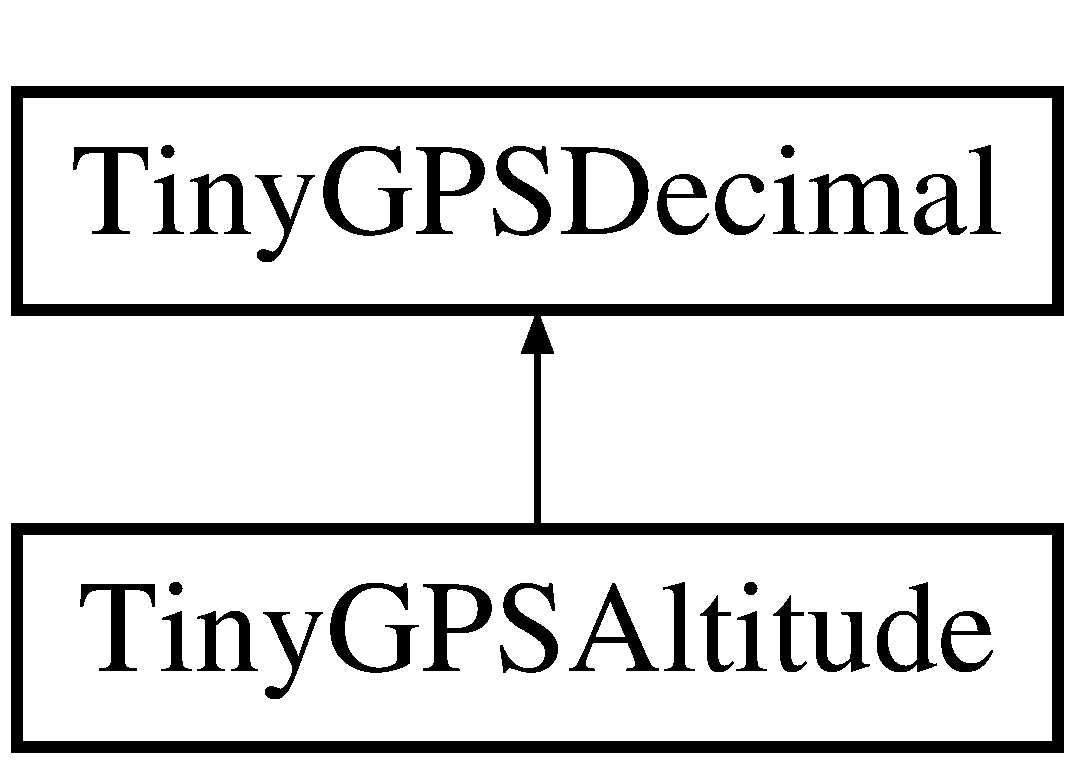
\includegraphics[height=2.000000cm]{struct_tiny_g_p_s_altitude}
\end{center}
\end{figure}
\subsection*{Public Member Functions}
\begin{DoxyCompactItemize}
\item 
double {\bfseries meters} ()\label{struct_tiny_g_p_s_altitude_a5a39d145bb1778814007206c765189f7}

\item 
double {\bfseries miles} ()\label{struct_tiny_g_p_s_altitude_a5ae68d990ea08d4e21cfa6aefb46cc03}

\item 
double {\bfseries kilometers} ()\label{struct_tiny_g_p_s_altitude_a1eb3e5b425784fc0db3e9ffe0f77f741}

\item 
double {\bfseries feet} ()\label{struct_tiny_g_p_s_altitude_ac782babc0c485d47e6f57384e88b8cc8}

\end{DoxyCompactItemize}


The documentation for this struct was generated from the following file\+:\begin{DoxyCompactItemize}
\item 
headers/Tiny\+G\+P\+S++.\+h\end{DoxyCompactItemize}

\section{Tiny\+G\+P\+S\+Course Struct Reference}
\label{struct_tiny_g_p_s_course}\index{Tiny\+G\+P\+S\+Course@{Tiny\+G\+P\+S\+Course}}
Inheritance diagram for Tiny\+G\+P\+S\+Course\+:\begin{figure}[H]
\begin{center}
\leavevmode
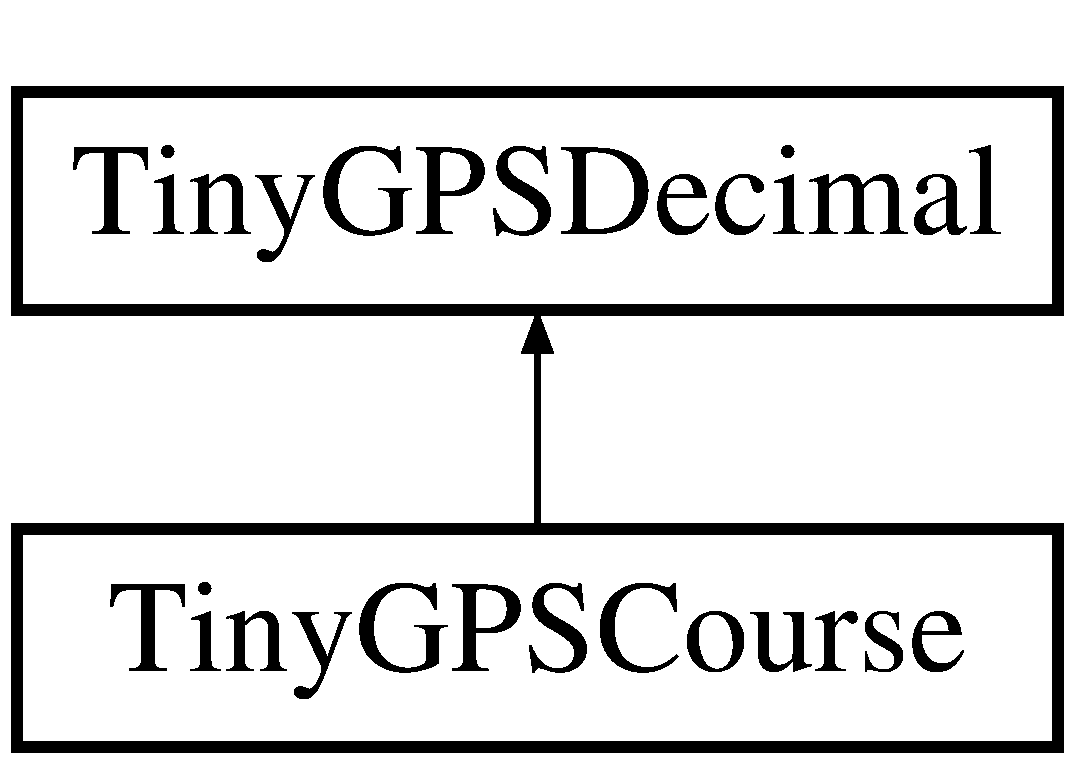
\includegraphics[height=2.000000cm]{struct_tiny_g_p_s_course}
\end{center}
\end{figure}
\subsection*{Public Member Functions}
\begin{DoxyCompactItemize}
\item 
double {\bfseries deg} ()\label{struct_tiny_g_p_s_course_a76dc8ae6c2fe5ead9b44c8d53a3272ca}

\end{DoxyCompactItemize}


The documentation for this struct was generated from the following file\+:\begin{DoxyCompactItemize}
\item 
headers/Tiny\+G\+P\+S++.\+h\end{DoxyCompactItemize}

\section{Tiny\+G\+P\+S\+Custom Class Reference}
\label{class_tiny_g_p_s_custom}\index{Tiny\+G\+P\+S\+Custom@{Tiny\+G\+P\+S\+Custom}}
\subsection*{Public Member Functions}
\begin{DoxyCompactItemize}
\item 
{\bfseries Tiny\+G\+P\+S\+Custom} ({\bf Tiny\+G\+P\+S\+Plus} \&gps, const char $\ast$sentence\+Name, int term\+Number)\label{class_tiny_g_p_s_custom_a29b2a658bf95d8e6265e983b1c0251b5}

\item 
void {\bfseries begin} ({\bf Tiny\+G\+P\+S\+Plus} \&gps, const char $\ast$\+\_\+sentence\+Name, int \+\_\+term\+Number)\label{class_tiny_g_p_s_custom_a3bf972f7e2e7e3f483071630e5ca8355}

\item 
bool {\bfseries is\+Updated} () const \label{class_tiny_g_p_s_custom_a3905509b3f88d67e248855c135744b14}

\item 
bool {\bfseries is\+Valid} () const \label{class_tiny_g_p_s_custom_a06fad8448c014424bf96ed379b55da21}

\item 
uint32\+\_\+t {\bfseries age} () const \label{class_tiny_g_p_s_custom_a9bacaf774b1dba9ad942435d3ed1c2cc}

\item 
const char $\ast$ {\bfseries value} ()\label{class_tiny_g_p_s_custom_ac5ad40a3d9b6fe386b2309f972566674}

\end{DoxyCompactItemize}
\subsection*{Friends}
\begin{DoxyCompactItemize}
\item 
class {\bfseries Tiny\+G\+P\+S\+Plus}\label{class_tiny_g_p_s_custom_a6501fd5ef19ae166d43e0e5781609ee2}

\end{DoxyCompactItemize}


The documentation for this class was generated from the following file\+:\begin{DoxyCompactItemize}
\item 
headers/Tiny\+G\+P\+S++.\+h\end{DoxyCompactItemize}

\hypertarget{struct_tiny_g_p_s_date}{}\section{Tiny\+G\+P\+S\+Date Struct Reference}
\label{struct_tiny_g_p_s_date}\index{Tiny\+G\+P\+S\+Date@{Tiny\+G\+P\+S\+Date}}
\subsection*{Public Member Functions}
\begin{DoxyCompactItemize}
\item 
bool {\bfseries is\+Valid} () const \hypertarget{struct_tiny_g_p_s_date_a0ef145848ab03e4e9db0e2cf3a4c42cd}{}\label{struct_tiny_g_p_s_date_a0ef145848ab03e4e9db0e2cf3a4c42cd}

\item 
bool {\bfseries is\+Updated} () const \hypertarget{struct_tiny_g_p_s_date_aed8706c1c3e67558fec2b94476c144e0}{}\label{struct_tiny_g_p_s_date_aed8706c1c3e67558fec2b94476c144e0}

\item 
uint32\+\_\+t {\bfseries age} () const \hypertarget{struct_tiny_g_p_s_date_a7b92ac9058dbde1770eb52ce5da890c1}{}\label{struct_tiny_g_p_s_date_a7b92ac9058dbde1770eb52ce5da890c1}

\item 
uint32\+\_\+t {\bfseries value} ()\hypertarget{struct_tiny_g_p_s_date_a718150ae16f68afa9ae81f9d1b3ce3f4}{}\label{struct_tiny_g_p_s_date_a718150ae16f68afa9ae81f9d1b3ce3f4}

\item 
uint16\+\_\+t {\bfseries year} ()\hypertarget{struct_tiny_g_p_s_date_ae2cc914fec377b429d99f01204f50d60}{}\label{struct_tiny_g_p_s_date_ae2cc914fec377b429d99f01204f50d60}

\item 
uint8\+\_\+t {\bfseries month} ()\hypertarget{struct_tiny_g_p_s_date_a6f3c5b4e72ef28b010f94ac9016315f3}{}\label{struct_tiny_g_p_s_date_a6f3c5b4e72ef28b010f94ac9016315f3}

\item 
uint8\+\_\+t {\bfseries day} ()\hypertarget{struct_tiny_g_p_s_date_ae8cc5f80c49e328f792d168a44062000}{}\label{struct_tiny_g_p_s_date_ae8cc5f80c49e328f792d168a44062000}

\end{DoxyCompactItemize}
\subsection*{Friends}
\begin{DoxyCompactItemize}
\item 
class {\bfseries Tiny\+G\+P\+S\+Plus}\hypertarget{struct_tiny_g_p_s_date_a6501fd5ef19ae166d43e0e5781609ee2}{}\label{struct_tiny_g_p_s_date_a6501fd5ef19ae166d43e0e5781609ee2}

\end{DoxyCompactItemize}


The documentation for this struct was generated from the following file\+:\begin{DoxyCompactItemize}
\item 
headers/Tiny\+G\+P\+S++.\+h\end{DoxyCompactItemize}

\hypertarget{struct_tiny_g_p_s_decimal}{}\section{Tiny\+G\+P\+S\+Decimal Struct Reference}
\label{struct_tiny_g_p_s_decimal}\index{Tiny\+G\+P\+S\+Decimal@{Tiny\+G\+P\+S\+Decimal}}
Inheritance diagram for Tiny\+G\+P\+S\+Decimal\+:\begin{figure}[H]
\begin{center}
\leavevmode
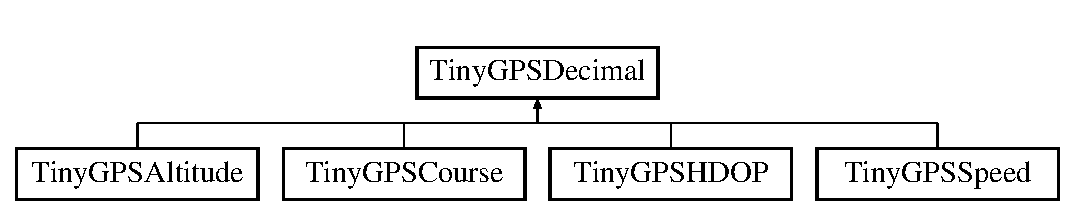
\includegraphics[height=2.000000cm]{struct_tiny_g_p_s_decimal}
\end{center}
\end{figure}
\subsection*{Public Member Functions}
\begin{DoxyCompactItemize}
\item 
bool {\bfseries is\+Valid} () const \hypertarget{struct_tiny_g_p_s_decimal_a2a1d868525e903eb193b7a36cdd76984}{}\label{struct_tiny_g_p_s_decimal_a2a1d868525e903eb193b7a36cdd76984}

\item 
bool {\bfseries is\+Updated} () const \hypertarget{struct_tiny_g_p_s_decimal_ae8b7f9f7719c2974ebd3b34759493d15}{}\label{struct_tiny_g_p_s_decimal_ae8b7f9f7719c2974ebd3b34759493d15}

\item 
uint32\+\_\+t {\bfseries age} () const \hypertarget{struct_tiny_g_p_s_decimal_ab80191a3e02c92ad3f674b5df2ab752f}{}\label{struct_tiny_g_p_s_decimal_ab80191a3e02c92ad3f674b5df2ab752f}

\item 
int32\+\_\+t {\bfseries value} ()\hypertarget{struct_tiny_g_p_s_decimal_ac3ce80976e5d8456e9f211b910a6cb19}{}\label{struct_tiny_g_p_s_decimal_ac3ce80976e5d8456e9f211b910a6cb19}

\end{DoxyCompactItemize}
\subsection*{Friends}
\begin{DoxyCompactItemize}
\item 
class {\bfseries Tiny\+G\+P\+S\+Plus}\hypertarget{struct_tiny_g_p_s_decimal_a6501fd5ef19ae166d43e0e5781609ee2}{}\label{struct_tiny_g_p_s_decimal_a6501fd5ef19ae166d43e0e5781609ee2}

\end{DoxyCompactItemize}


The documentation for this struct was generated from the following file\+:\begin{DoxyCompactItemize}
\item 
headers/Tiny\+G\+P\+S++.\+h\end{DoxyCompactItemize}

\section{Tiny\+G\+P\+S\+H\+D\+OP Struct Reference}
\label{struct_tiny_g_p_s_h_d_o_p}\index{Tiny\+G\+P\+S\+H\+D\+OP@{Tiny\+G\+P\+S\+H\+D\+OP}}
Inheritance diagram for Tiny\+G\+P\+S\+H\+D\+OP\+:\begin{figure}[H]
\begin{center}
\leavevmode
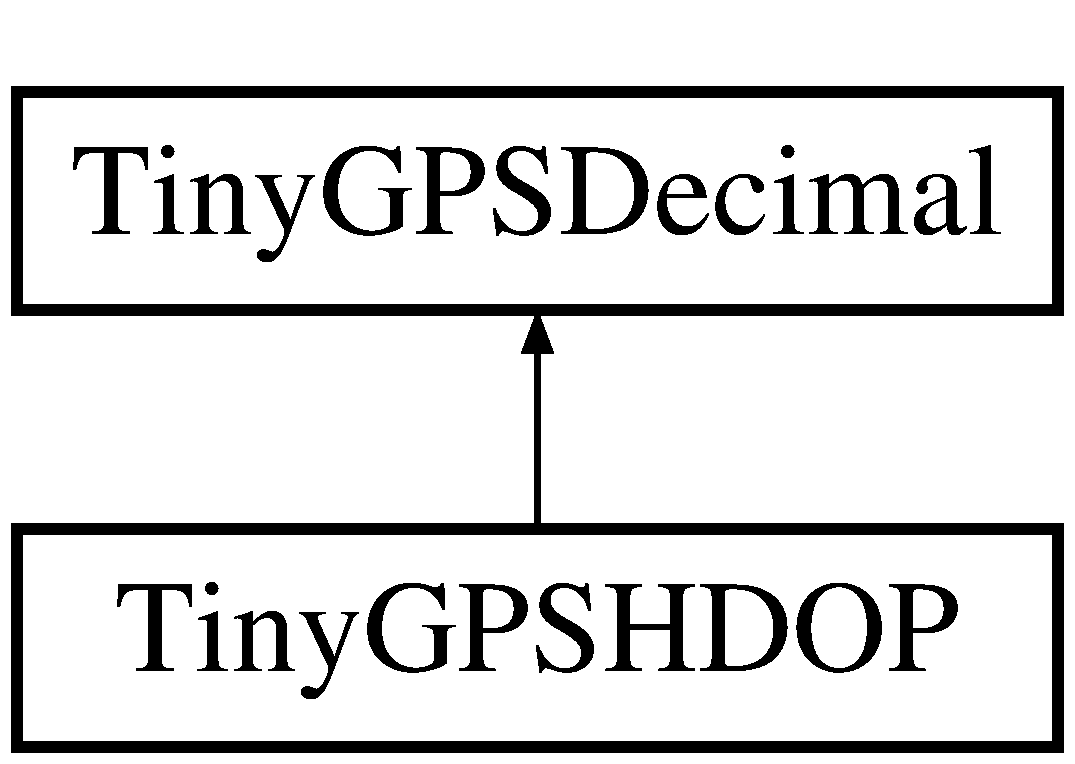
\includegraphics[height=2.000000cm]{struct_tiny_g_p_s_h_d_o_p}
\end{center}
\end{figure}
\subsection*{Public Member Functions}
\begin{DoxyCompactItemize}
\item 
double {\bfseries hdop} ()\label{struct_tiny_g_p_s_h_d_o_p_a27cd35588c96eefb690bba46497d20d7}

\end{DoxyCompactItemize}


The documentation for this struct was generated from the following file\+:\begin{DoxyCompactItemize}
\item 
headers/Tiny\+G\+P\+S++.\+h\end{DoxyCompactItemize}

\section{Tiny\+G\+P\+S\+Integer Struct Reference}
\label{struct_tiny_g_p_s_integer}\index{Tiny\+G\+P\+S\+Integer@{Tiny\+G\+P\+S\+Integer}}
\subsection*{Public Member Functions}
\begin{DoxyCompactItemize}
\item 
bool {\bfseries is\+Valid} () const \label{struct_tiny_g_p_s_integer_aad411b5eb6cc16774ff0ff8d275df2fa}

\item 
bool {\bfseries is\+Updated} () const \label{struct_tiny_g_p_s_integer_aa6479670272df580287f84938183dc20}

\item 
uint32\+\_\+t {\bfseries age} () const \label{struct_tiny_g_p_s_integer_a46ea8f4fe8cca279b7d4cd44572e5881}

\item 
uint32\+\_\+t {\bfseries value} ()\label{struct_tiny_g_p_s_integer_a67de7e76d61dbd25eb32f701d8ce867b}

\end{DoxyCompactItemize}
\subsection*{Friends}
\begin{DoxyCompactItemize}
\item 
class {\bfseries Tiny\+G\+P\+S\+Plus}\label{struct_tiny_g_p_s_integer_a6501fd5ef19ae166d43e0e5781609ee2}

\end{DoxyCompactItemize}


The documentation for this struct was generated from the following file\+:\begin{DoxyCompactItemize}
\item 
headers/Tiny\+G\+P\+S++.\+h\end{DoxyCompactItemize}

\section{Tiny\+G\+P\+S\+Location Struct Reference}
\label{struct_tiny_g_p_s_location}\index{Tiny\+G\+P\+S\+Location@{Tiny\+G\+P\+S\+Location}}
\subsection*{Public Member Functions}
\begin{DoxyCompactItemize}
\item 
bool {\bfseries is\+Valid} () const \label{struct_tiny_g_p_s_location_a783c2898915440f51a6df233aba51923}

\item 
bool {\bfseries is\+Updated} () const \label{struct_tiny_g_p_s_location_a9aae0a5fd73c2dab231309f1dd3b2c0a}

\item 
uint32\+\_\+t {\bfseries age} () const \label{struct_tiny_g_p_s_location_ada111e1b74f82dc029c0c61241424ca8}

\item 
const {\bf Raw\+Degrees} \& {\bfseries raw\+Lat} ()\label{struct_tiny_g_p_s_location_abe2a4fbfe28299aae87c5b4c3c58bcad}

\item 
const {\bf Raw\+Degrees} \& {\bfseries raw\+Lng} ()\label{struct_tiny_g_p_s_location_a9fe126feca0bdcfa9224a428b86d68db}

\item 
double {\bfseries lat} ()\label{struct_tiny_g_p_s_location_a86c3acea4f317b427eebb667e4d05a49}

\item 
double {\bfseries lng} ()\label{struct_tiny_g_p_s_location_a544e9009a5580b2fd5466821a5e5b782}

\end{DoxyCompactItemize}
\subsection*{Friends}
\begin{DoxyCompactItemize}
\item 
class {\bfseries Tiny\+G\+P\+S\+Plus}\label{struct_tiny_g_p_s_location_a6501fd5ef19ae166d43e0e5781609ee2}

\end{DoxyCompactItemize}


The documentation for this struct was generated from the following file\+:\begin{DoxyCompactItemize}
\item 
headers/Tiny\+G\+P\+S++.\+h\end{DoxyCompactItemize}

\section{Tiny\+G\+P\+S\+Plus Class Reference}
\label{class_tiny_g_p_s_plus}\index{Tiny\+G\+P\+S\+Plus@{Tiny\+G\+P\+S\+Plus}}
\subsection*{Public Member Functions}
\begin{DoxyCompactItemize}
\item 
bool {\bfseries encode} (char c)\label{class_tiny_g_p_s_plus_ad7b78320b7e4967df17c6a27008a5154}

\item 
{\bf Tiny\+G\+P\+S\+Plus} \& {\bfseries operator$<$$<$} (char c)\label{class_tiny_g_p_s_plus_a32a0b61a25ce0c490216cb2b4ea19ced}

\item 
uint32\+\_\+t {\bfseries chars\+Processed} () const \label{class_tiny_g_p_s_plus_a12b6bc0169ee6b2f0beb8041e549f338}

\item 
uint32\+\_\+t {\bfseries sentences\+With\+Fix} () const \label{class_tiny_g_p_s_plus_a6c502ec591dc42a83771a502c4dbdcd4}

\item 
uint32\+\_\+t {\bfseries failed\+Checksum} () const \label{class_tiny_g_p_s_plus_a57dd7a4430d58f784e967ee2d76e574f}

\item 
uint32\+\_\+t {\bfseries passed\+Checksum} () const \label{class_tiny_g_p_s_plus_a55af5d3442bf8f5c5fdd0309e416d9e5}

\end{DoxyCompactItemize}
\subsection*{Static Public Member Functions}
\begin{DoxyCompactItemize}
\item 
static const char $\ast$ {\bfseries library\+Version} ()\label{class_tiny_g_p_s_plus_a1ec39648e1c80c59f4fded642fdb88ae}

\item 
static double {\bfseries distance\+Between} (double lat1, double long1, double lat2, double long2)\label{class_tiny_g_p_s_plus_add9aef227cf2836b53cbdfed5133bb4d}

\item 
static double {\bfseries course\+To} (double lat1, double long1, double lat2, double long2)\label{class_tiny_g_p_s_plus_a82b8fff820573de45c9ae98df3abbdfa}

\item 
static const char $\ast$ {\bfseries cardinal} (double course)\label{class_tiny_g_p_s_plus_a68029db9475edf20c750eb0b7a6f1118}

\item 
static int32\+\_\+t {\bfseries parse\+Decimal} (const char $\ast$term)\label{class_tiny_g_p_s_plus_afd333e29a6a337affc6531183d716e04}

\item 
static void {\bfseries parse\+Degrees} (const char $\ast$term, {\bf Raw\+Degrees} \&deg)\label{class_tiny_g_p_s_plus_ad17b86db786450c5c7249aba98090954}

\end{DoxyCompactItemize}
\subsection*{Public Attributes}
\begin{DoxyCompactItemize}
\item 
{\bf Tiny\+G\+P\+S\+Location} {\bfseries location}\label{class_tiny_g_p_s_plus_a886255f412f8e01f84e5104d36315fb3}

\item 
{\bf Tiny\+G\+P\+S\+Date} {\bfseries date}\label{class_tiny_g_p_s_plus_a83a70812b432d7f51c7c735bfe7be0f0}

\item 
{\bf Tiny\+G\+P\+S\+Time} {\bfseries time}\label{class_tiny_g_p_s_plus_a377c975527fa24b45fb86356505eb134}

\item 
{\bf Tiny\+G\+P\+S\+Speed} {\bfseries speed}\label{class_tiny_g_p_s_plus_aa085c3e72a399a829dd92af52b373404}

\item 
{\bf Tiny\+G\+P\+S\+Course} {\bfseries course}\label{class_tiny_g_p_s_plus_ad7800d3decbe58e355f5229bba231868}

\item 
{\bf Tiny\+G\+P\+S\+Altitude} {\bfseries altitude}\label{class_tiny_g_p_s_plus_a0b3451a4ee75e5880ffd88c3038eacf8}

\item 
{\bf Tiny\+G\+P\+S\+Integer} {\bfseries satellites}\label{class_tiny_g_p_s_plus_a5fb47066d1d03f4bb5853529053aab48}

\item 
{\bf Tiny\+G\+P\+S\+H\+D\+OP} {\bfseries hdop}\label{class_tiny_g_p_s_plus_a0bb6a7eb2d0261095911d71c8c067546}

\end{DoxyCompactItemize}
\subsection*{Friends}
\begin{DoxyCompactItemize}
\item 
class {\bfseries Tiny\+G\+P\+S\+Custom}\label{class_tiny_g_p_s_plus_aaad5bf5a2728a81e624ad2304f817772}

\end{DoxyCompactItemize}


The documentation for this class was generated from the following file\+:\begin{DoxyCompactItemize}
\item 
headers/Tiny\+G\+P\+S++.\+h\end{DoxyCompactItemize}

\section{Tiny\+G\+P\+S\+Speed Struct Reference}
\label{struct_tiny_g_p_s_speed}\index{Tiny\+G\+P\+S\+Speed@{Tiny\+G\+P\+S\+Speed}}
Inheritance diagram for Tiny\+G\+P\+S\+Speed\+:\begin{figure}[H]
\begin{center}
\leavevmode
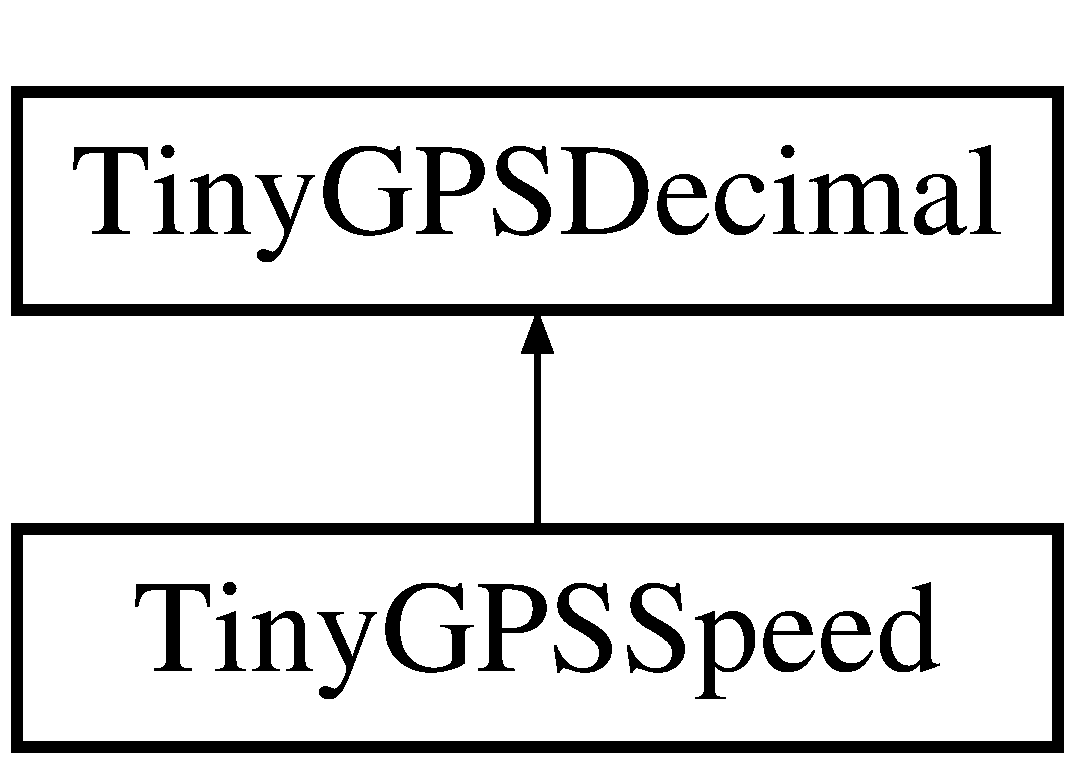
\includegraphics[height=2.000000cm]{struct_tiny_g_p_s_speed}
\end{center}
\end{figure}
\subsection*{Public Member Functions}
\begin{DoxyCompactItemize}
\item 
double {\bfseries knots} ()\label{struct_tiny_g_p_s_speed_aa3a38ce4ece3d8062c794b73f260395e}

\item 
double {\bfseries mph} ()\label{struct_tiny_g_p_s_speed_a1809120167961ea9a85e860a964b1c6e}

\item 
double {\bfseries mps} ()\label{struct_tiny_g_p_s_speed_aacee536241e810cdf4ba7846d6c202cb}

\item 
double {\bfseries kmph} ()\label{struct_tiny_g_p_s_speed_a7fee3c8f9f2fcc5f4a517bd6108f79dd}

\end{DoxyCompactItemize}


The documentation for this struct was generated from the following file\+:\begin{DoxyCompactItemize}
\item 
headers/Tiny\+G\+P\+S++.\+h\end{DoxyCompactItemize}

\hypertarget{struct_tiny_g_p_s_time}{}\section{Tiny\+G\+P\+S\+Time Struct Reference}
\label{struct_tiny_g_p_s_time}\index{Tiny\+G\+P\+S\+Time@{Tiny\+G\+P\+S\+Time}}
\subsection*{Public Member Functions}
\begin{DoxyCompactItemize}
\item 
bool {\bfseries is\+Valid} () const \hypertarget{struct_tiny_g_p_s_time_a85c38acaf804aecefc3f0358bf93d86a}{}\label{struct_tiny_g_p_s_time_a85c38acaf804aecefc3f0358bf93d86a}

\item 
bool {\bfseries is\+Updated} () const \hypertarget{struct_tiny_g_p_s_time_a48850598e5ae6dd6813bbfd5af7589fc}{}\label{struct_tiny_g_p_s_time_a48850598e5ae6dd6813bbfd5af7589fc}

\item 
uint32\+\_\+t {\bfseries age} () const \hypertarget{struct_tiny_g_p_s_time_a22b59e1d4b22435baa2a4446981f2dce}{}\label{struct_tiny_g_p_s_time_a22b59e1d4b22435baa2a4446981f2dce}

\item 
uint32\+\_\+t {\bfseries value} ()\hypertarget{struct_tiny_g_p_s_time_afcdb632fee9d144b1414c9d7b95719f1}{}\label{struct_tiny_g_p_s_time_afcdb632fee9d144b1414c9d7b95719f1}

\item 
uint8\+\_\+t {\bfseries hour} ()\hypertarget{struct_tiny_g_p_s_time_a37fdb629b6ed0e31134214c7d07df2b1}{}\label{struct_tiny_g_p_s_time_a37fdb629b6ed0e31134214c7d07df2b1}

\item 
uint8\+\_\+t {\bfseries minute} ()\hypertarget{struct_tiny_g_p_s_time_aef83c20c14d404219299da2d7e35cdce}{}\label{struct_tiny_g_p_s_time_aef83c20c14d404219299da2d7e35cdce}

\item 
uint8\+\_\+t {\bfseries second} ()\hypertarget{struct_tiny_g_p_s_time_a729cab36ced07eb5607503663fbe33e8}{}\label{struct_tiny_g_p_s_time_a729cab36ced07eb5607503663fbe33e8}

\item 
uint8\+\_\+t {\bfseries centisecond} ()\hypertarget{struct_tiny_g_p_s_time_a1f74ad4a2a53e0ee19f8e3a6b2bc985f}{}\label{struct_tiny_g_p_s_time_a1f74ad4a2a53e0ee19f8e3a6b2bc985f}

\end{DoxyCompactItemize}
\subsection*{Friends}
\begin{DoxyCompactItemize}
\item 
class {\bfseries Tiny\+G\+P\+S\+Plus}\hypertarget{struct_tiny_g_p_s_time_a6501fd5ef19ae166d43e0e5781609ee2}{}\label{struct_tiny_g_p_s_time_a6501fd5ef19ae166d43e0e5781609ee2}

\end{DoxyCompactItemize}


The documentation for this struct was generated from the following file\+:\begin{DoxyCompactItemize}
\item 
headers/Tiny\+G\+P\+S++.\+h\end{DoxyCompactItemize}

\section{T\+WI Class Reference}
\label{class_t_w_i}\index{T\+WI@{T\+WI}}
\subsection*{Public Member Functions}
\begin{DoxyCompactItemize}
\item 
{\bf T\+WI} (int freq)
\item 
bool {\bf send\+Start} ()
\item 
bool {\bf send\+Repeated\+Start} ()
\item 
void {\bf send\+Stop} ()
\item 
bool {\bf send\+Read\+Address} (byte address)
\item 
bool {\bf send\+Write\+Address} (byte address)
\item 
bool {\bf send\+Data} (byte dado)
\item 
bool {\bf read\+Data} (bool ack, uint8\+\_\+t $\ast$data)
\end{DoxyCompactItemize}


\subsection{Constructor \& Destructor Documentation}
\index{T\+WI@{T\+WI}!T\+WI@{T\+WI}}
\index{T\+WI@{T\+WI}!T\+WI@{T\+WI}}
\subsubsection[{T\+W\+I(int freq)}]{\setlength{\rightskip}{0pt plus 5cm}T\+W\+I\+::\+T\+WI (
\begin{DoxyParamCaption}
\item[{int}]{freq}
\end{DoxyParamCaption}
)}\label{class_t_w_i_a055a0378dde5773bf5909055d05b735b}
Construtor da classe. Define a frequência que vai ser trabalhada e o endereço do escravo. 
\begin{DoxyParams}{Parameters}
{\em freq} & frequência utilizada \\
\hline
\end{DoxyParams}


\subsection{Member Function Documentation}
\index{T\+WI@{T\+WI}!read\+Data@{read\+Data}}
\index{read\+Data@{read\+Data}!T\+WI@{T\+WI}}
\subsubsection[{read\+Data(bool ack, uint8\+\_\+t $\ast$data)}]{\setlength{\rightskip}{0pt plus 5cm}bool T\+W\+I\+::read\+Data (
\begin{DoxyParamCaption}
\item[{bool}]{ack, }
\item[{uint8\+\_\+t $\ast$}]{data}
\end{DoxyParamCaption}
)}\label{class_t_w_i_ab22fbccf340064182a0fa99447ec0eef}
Lê um dado. 
\begin{DoxyParams}{Parameters}
{\em ack} & determina se quer receber A\+CK (T\+R\+UE) ou N\+A\+CK (F\+A\+L\+SE) \\
\hline
{\em data} & byte lido \\
\hline
\end{DoxyParams}
\begin{DoxyReturn}{Returns}
T\+R\+UE se ocorreu tudo bem, F\+A\+L\+SE caso contrario 
\end{DoxyReturn}
\index{T\+WI@{T\+WI}!send\+Data@{send\+Data}}
\index{send\+Data@{send\+Data}!T\+WI@{T\+WI}}
\subsubsection[{send\+Data(byte dado)}]{\setlength{\rightskip}{0pt plus 5cm}bool T\+W\+I\+::send\+Data (
\begin{DoxyParamCaption}
\item[{byte}]{dado}
\end{DoxyParamCaption}
)}\label{class_t_w_i_a90bcdbb964dc3876cf8876d8ba579964}
Envia um dado. 
\begin{DoxyParams}{Parameters}
{\em dado} & dado que vai ser enviado \\
\hline
\end{DoxyParams}
\begin{DoxyReturn}{Returns}
T\+R\+UE se o dado foi enviado e F\+A\+L\+SE caso contrário 
\end{DoxyReturn}
\index{T\+WI@{T\+WI}!send\+Read\+Address@{send\+Read\+Address}}
\index{send\+Read\+Address@{send\+Read\+Address}!T\+WI@{T\+WI}}
\subsubsection[{send\+Read\+Address(byte address)}]{\setlength{\rightskip}{0pt plus 5cm}bool T\+W\+I\+::send\+Read\+Address (
\begin{DoxyParamCaption}
\item[{byte}]{address}
\end{DoxyParamCaption}
)}\label{class_t_w_i_a4f26411a5da8111232c91c70f06048cd}
Envia o endereço de leitura. 
\begin{DoxyParams}{Parameters}
{\em address} & endereço de leitura \\
\hline
\end{DoxyParams}
\begin{DoxyReturn}{Returns}
T\+R\+UE se endereço foi enviado e F\+A\+L\+SE caso contrário 
\end{DoxyReturn}
\index{T\+WI@{T\+WI}!send\+Repeated\+Start@{send\+Repeated\+Start}}
\index{send\+Repeated\+Start@{send\+Repeated\+Start}!T\+WI@{T\+WI}}
\subsubsection[{send\+Repeated\+Start()}]{\setlength{\rightskip}{0pt plus 5cm}bool T\+W\+I\+::send\+Repeated\+Start (
\begin{DoxyParamCaption}
{}
\end{DoxyParamCaption}
)}\label{class_t_w_i_a88fe10bf711a21b84b1e688e8c9ad726}
Envia um sinal de start repetido. Caso falhe, repete R\+E\+P\+E\+A\+T\+\_\+\+S\+T\+A\+RT vezes. \begin{DoxyReturn}{Returns}
T\+R\+UE se start repetido ocorreu e F\+A\+L\+SE caso contrário 
\end{DoxyReturn}
\index{T\+WI@{T\+WI}!send\+Start@{send\+Start}}
\index{send\+Start@{send\+Start}!T\+WI@{T\+WI}}
\subsubsection[{send\+Start()}]{\setlength{\rightskip}{0pt plus 5cm}bool T\+W\+I\+::send\+Start (
\begin{DoxyParamCaption}
{}
\end{DoxyParamCaption}
)}\label{class_t_w_i_ac9cb5ceb7c069342e6c106117fa50c92}
Envia um sinal de start. Caso falhe, repete R\+E\+P\+E\+A\+T\+\_\+\+S\+T\+A\+RT vezes. \begin{DoxyReturn}{Returns}
T\+R\+UE se start ocorreu e F\+A\+L\+SE caso contrário 
\end{DoxyReturn}
\index{T\+WI@{T\+WI}!send\+Stop@{send\+Stop}}
\index{send\+Stop@{send\+Stop}!T\+WI@{T\+WI}}
\subsubsection[{send\+Stop()}]{\setlength{\rightskip}{0pt plus 5cm}void T\+W\+I\+::send\+Stop (
\begin{DoxyParamCaption}
{}
\end{DoxyParamCaption}
)}\label{class_t_w_i_a34828bccdff0c441ffbb1d57e724d7d0}
Envia um sinal de stop. \index{T\+WI@{T\+WI}!send\+Write\+Address@{send\+Write\+Address}}
\index{send\+Write\+Address@{send\+Write\+Address}!T\+WI@{T\+WI}}
\subsubsection[{send\+Write\+Address(byte address)}]{\setlength{\rightskip}{0pt plus 5cm}bool T\+W\+I\+::send\+Write\+Address (
\begin{DoxyParamCaption}
\item[{byte}]{address}
\end{DoxyParamCaption}
)}\label{class_t_w_i_aada3a61390b78a34c51565ecf534e0b4}
Envia o endereço de escrita. 
\begin{DoxyParams}{Parameters}
{\em address} & endereço de escrita \\
\hline
\end{DoxyParams}
\begin{DoxyReturn}{Returns}
T\+R\+UE se endereço foi enviado e F\+A\+L\+SE caso contrário 
\end{DoxyReturn}


The documentation for this class was generated from the following file\+:\begin{DoxyCompactItemize}
\item 
headers/T\+W\+I.\+h\end{DoxyCompactItemize}

\hypertarget{class_u_s_a_r_t}{}\section{U\+S\+A\+RT Class Reference}
\label{class_u_s_a_r_t}\index{U\+S\+A\+RT@{U\+S\+A\+RT}}
\subsection*{Public Member Functions}
\begin{DoxyCompactItemize}
\item 
\hyperlink{class_u_s_a_r_t_a538ccfb4c4ae821f4fd4e87afe9fd96e}{U\+S\+A\+RT} ()
\item 
\hyperlink{class_u_s_a_r_t_a680846cecf681784c7a113d145104c5d}{U\+S\+A\+RT} (int serial\+Number, long baud\+Rate)
\item 
byte \hyperlink{class_u_s_a_r_t_afdd6c6b8cc0b12375978e492f9eeefca}{read\+Byte} ()
\item 
void \hyperlink{class_u_s_a_r_t_aa1c1e5fef5153dd3d4d2794e16433b3f}{print} (char dado\mbox{[}$\,$\mbox{]})
\item 
void \hyperlink{class_u_s_a_r_t_a85c5f9ee155061a1c34bef668c7858e7}{print} (long dado)
\item 
void \hyperlink{class_u_s_a_r_t_aaf26f0a495fa3248035bec99f6871969}{print} (int dado)
\item 
void \hyperlink{class_u_s_a_r_t_a93d4b2375905a82d459bf243d336fbe8}{print} (double dado)
\item 
void \hyperlink{class_u_s_a_r_t_ad80fac8322685697839dfb8a85d52d94}{print} (word dado, int modo=D\+EC)
\item 
void \hyperlink{class_u_s_a_r_t_a247454f341ef377b168436fca1490861}{print} (byte dado, int modo=D\+EC)
\item 
void \hyperlink{class_u_s_a_r_t_ab7a2d9febdda04636cf13ccc2d004475}{println} (char dado\mbox{[}$\,$\mbox{]})
\item 
void \hyperlink{class_u_s_a_r_t_af466ae5e7c9f85ed409274a15c08d69a}{println} (long dado)
\item 
void \hyperlink{class_u_s_a_r_t_a4c59a4f57021fcf5bae5e8a3a963d4e3}{println} (int dado)
\item 
void \hyperlink{class_u_s_a_r_t_a93e3e2c0822214f5cd9f3d65d87400ec}{println} (double dado)
\item 
void \hyperlink{class_u_s_a_r_t_ac554e6cd095025857ab747c63e407454}{println} (word dado, int modo=D\+EC)
\item 
void \hyperlink{class_u_s_a_r_t_ae6893c448241c72ddf6867034657c4c5}{println} (byte dado, int modo=D\+EC)
\end{DoxyCompactItemize}


\subsection{Constructor \& Destructor Documentation}
\index{U\+S\+A\+RT@{U\+S\+A\+RT}!U\+S\+A\+RT@{U\+S\+A\+RT}}
\index{U\+S\+A\+RT@{U\+S\+A\+RT}!U\+S\+A\+RT@{U\+S\+A\+RT}}
\subsubsection[{\texorpdfstring{U\+S\+A\+R\+T()}{USART()}}]{\setlength{\rightskip}{0pt plus 5cm}U\+S\+A\+R\+T\+::\+U\+S\+A\+RT (
\begin{DoxyParamCaption}
{}
\end{DoxyParamCaption}
)}\hypertarget{class_u_s_a_r_t_a538ccfb4c4ae821f4fd4e87afe9fd96e}{}\label{class_u_s_a_r_t_a538ccfb4c4ae821f4fd4e87afe9fd96e}
Construtor default da classe. \index{U\+S\+A\+RT@{U\+S\+A\+RT}!U\+S\+A\+RT@{U\+S\+A\+RT}}
\index{U\+S\+A\+RT@{U\+S\+A\+RT}!U\+S\+A\+RT@{U\+S\+A\+RT}}
\subsubsection[{\texorpdfstring{U\+S\+A\+R\+T(int serial\+Number, long baud\+Rate)}{USART(int serialNumber, long baudRate)}}]{\setlength{\rightskip}{0pt plus 5cm}U\+S\+A\+R\+T\+::\+U\+S\+A\+RT (
\begin{DoxyParamCaption}
\item[{int}]{serial\+Number, }
\item[{long}]{baud\+Rate}
\end{DoxyParamCaption}
)}\hypertarget{class_u_s_a_r_t_a680846cecf681784c7a113d145104c5d}{}\label{class_u_s_a_r_t_a680846cecf681784c7a113d145104c5d}
Construtor da classe. Inicia uma comunicação serial em uma das portas do arduino utilizando o baud rate informado 
\begin{DoxyParams}{Parameters}
{\em serial\+Number} & qual porta serial será utilizada. No mega pode ser 0, 1, 2 ou 3 \\
\hline
{\em baud\+Rate} & baud Rate da comunicação. \\
\hline
\end{DoxyParams}


\subsection{Member Function Documentation}
\index{U\+S\+A\+RT@{U\+S\+A\+RT}!print@{print}}
\index{print@{print}!U\+S\+A\+RT@{U\+S\+A\+RT}}
\subsubsection[{\texorpdfstring{print(char dado[])}{print(char dado[])}}]{\setlength{\rightskip}{0pt plus 5cm}void U\+S\+A\+R\+T\+::print (
\begin{DoxyParamCaption}
\item[{char}]{dado\mbox{[}$\,$\mbox{]}}
\end{DoxyParamCaption}
)}\hypertarget{class_u_s_a_r_t_aa1c1e5fef5153dd3d4d2794e16433b3f}{}\label{class_u_s_a_r_t_aa1c1e5fef5153dd3d4d2794e16433b3f}
Imprime uma string 
\begin{DoxyParams}{Parameters}
{\em dado} & dado que será impresso \\
\hline
\end{DoxyParams}
\index{U\+S\+A\+RT@{U\+S\+A\+RT}!print@{print}}
\index{print@{print}!U\+S\+A\+RT@{U\+S\+A\+RT}}
\subsubsection[{\texorpdfstring{print(long dado)}{print(long dado)}}]{\setlength{\rightskip}{0pt plus 5cm}void U\+S\+A\+R\+T\+::print (
\begin{DoxyParamCaption}
\item[{long}]{dado}
\end{DoxyParamCaption}
)}\hypertarget{class_u_s_a_r_t_a85c5f9ee155061a1c34bef668c7858e7}{}\label{class_u_s_a_r_t_a85c5f9ee155061a1c34bef668c7858e7}
Imprime em decimal com sinal um long, retirando os zeros à esquerda 
\begin{DoxyParams}{Parameters}
{\em dado} & dado que será impresso \\
\hline
\end{DoxyParams}
\index{U\+S\+A\+RT@{U\+S\+A\+RT}!print@{print}}
\index{print@{print}!U\+S\+A\+RT@{U\+S\+A\+RT}}
\subsubsection[{\texorpdfstring{print(int dado)}{print(int dado)}}]{\setlength{\rightskip}{0pt plus 5cm}void U\+S\+A\+R\+T\+::print (
\begin{DoxyParamCaption}
\item[{int}]{dado}
\end{DoxyParamCaption}
)}\hypertarget{class_u_s_a_r_t_aaf26f0a495fa3248035bec99f6871969}{}\label{class_u_s_a_r_t_aaf26f0a495fa3248035bec99f6871969}
Imprime em decimal com sinal um int, retirando os zeros à esquerda 
\begin{DoxyParams}{Parameters}
{\em dado} & dado que será impresso \\
\hline
\end{DoxyParams}
\index{U\+S\+A\+RT@{U\+S\+A\+RT}!print@{print}}
\index{print@{print}!U\+S\+A\+RT@{U\+S\+A\+RT}}
\subsubsection[{\texorpdfstring{print(double dado)}{print(double dado)}}]{\setlength{\rightskip}{0pt plus 5cm}void U\+S\+A\+R\+T\+::print (
\begin{DoxyParamCaption}
\item[{double}]{dado}
\end{DoxyParamCaption}
)}\hypertarget{class_u_s_a_r_t_a93d4b2375905a82d459bf243d336fbe8}{}\label{class_u_s_a_r_t_a93d4b2375905a82d459bf243d336fbe8}
Imprime em double xx.\+xxxxxx 
\begin{DoxyParams}{Parameters}
{\em dado} & dado que será impresso \\
\hline
\end{DoxyParams}
\index{U\+S\+A\+RT@{U\+S\+A\+RT}!print@{print}}
\index{print@{print}!U\+S\+A\+RT@{U\+S\+A\+RT}}
\subsubsection[{\texorpdfstring{print(word dado, int modo=\+D\+E\+C)}{print(word dado, int modo=DEC)}}]{\setlength{\rightskip}{0pt plus 5cm}void U\+S\+A\+R\+T\+::print (
\begin{DoxyParamCaption}
\item[{word}]{dado, }
\item[{int}]{modo = {\ttfamily DEC}}
\end{DoxyParamCaption}
)}\hypertarget{class_u_s_a_r_t_ad80fac8322685697839dfb8a85d52d94}{}\label{class_u_s_a_r_t_ad80fac8322685697839dfb8a85d52d94}
Se o modo for decimal, imprime em decimal sem sinal um W16. Se o modo for hexadecimal, imprime em hexa um palavra de 16 bits. Possui como padrão o modo decimal. 
\begin{DoxyParams}{Parameters}
{\em dado} & dado que será impresso \\
\hline
{\em modo} & D\+EC para decimal e H\+EX para hexadecimal \\
\hline
\end{DoxyParams}
\index{U\+S\+A\+RT@{U\+S\+A\+RT}!print@{print}}
\index{print@{print}!U\+S\+A\+RT@{U\+S\+A\+RT}}
\subsubsection[{\texorpdfstring{print(byte dado, int modo=\+D\+E\+C)}{print(byte dado, int modo=DEC)}}]{\setlength{\rightskip}{0pt plus 5cm}void U\+S\+A\+R\+T\+::print (
\begin{DoxyParamCaption}
\item[{byte}]{dado, }
\item[{int}]{modo = {\ttfamily DEC}}
\end{DoxyParamCaption}
)}\hypertarget{class_u_s_a_r_t_a247454f341ef377b168436fca1490861}{}\label{class_u_s_a_r_t_a247454f341ef377b168436fca1490861}
Se o modo for decimal, imprime em decimal sem sinal um byte retirando os zeros à esquerda. Se o modo for hexadecimal, imprime em Hexa um byte. Possui como padrão o modo decimal. 
\begin{DoxyParams}{Parameters}
{\em dado} & dado que será impresso \\
\hline
{\em modo} & D\+EC para decimal e H\+EX para hexadecimal \\
\hline
\end{DoxyParams}
\index{U\+S\+A\+RT@{U\+S\+A\+RT}!println@{println}}
\index{println@{println}!U\+S\+A\+RT@{U\+S\+A\+RT}}
\subsubsection[{\texorpdfstring{println(char dado[])}{println(char dado[])}}]{\setlength{\rightskip}{0pt plus 5cm}void U\+S\+A\+R\+T\+::println (
\begin{DoxyParamCaption}
\item[{char}]{dado\mbox{[}$\,$\mbox{]}}
\end{DoxyParamCaption}
)}\hypertarget{class_u_s_a_r_t_ab7a2d9febdda04636cf13ccc2d004475}{}\label{class_u_s_a_r_t_ab7a2d9febdda04636cf13ccc2d004475}
Imprime uma string e pula uma linha 
\begin{DoxyParams}{Parameters}
{\em dado} & dado que será impresso \\
\hline
\end{DoxyParams}
\index{U\+S\+A\+RT@{U\+S\+A\+RT}!println@{println}}
\index{println@{println}!U\+S\+A\+RT@{U\+S\+A\+RT}}
\subsubsection[{\texorpdfstring{println(long dado)}{println(long dado)}}]{\setlength{\rightskip}{0pt plus 5cm}void U\+S\+A\+R\+T\+::println (
\begin{DoxyParamCaption}
\item[{long}]{dado}
\end{DoxyParamCaption}
)}\hypertarget{class_u_s_a_r_t_af466ae5e7c9f85ed409274a15c08d69a}{}\label{class_u_s_a_r_t_af466ae5e7c9f85ed409274a15c08d69a}
Imprime em decimal com sinal um long e pula uma linha 
\begin{DoxyParams}{Parameters}
{\em dado} & dado que será impresso \\
\hline
\end{DoxyParams}
\index{U\+S\+A\+RT@{U\+S\+A\+RT}!println@{println}}
\index{println@{println}!U\+S\+A\+RT@{U\+S\+A\+RT}}
\subsubsection[{\texorpdfstring{println(int dado)}{println(int dado)}}]{\setlength{\rightskip}{0pt plus 5cm}void U\+S\+A\+R\+T\+::println (
\begin{DoxyParamCaption}
\item[{int}]{dado}
\end{DoxyParamCaption}
)}\hypertarget{class_u_s_a_r_t_a4c59a4f57021fcf5bae5e8a3a963d4e3}{}\label{class_u_s_a_r_t_a4c59a4f57021fcf5bae5e8a3a963d4e3}
Imprime em decimal com sinal um int e pula uma linha 
\begin{DoxyParams}{Parameters}
{\em dado} & dado que será impresso \\
\hline
\end{DoxyParams}
\index{U\+S\+A\+RT@{U\+S\+A\+RT}!println@{println}}
\index{println@{println}!U\+S\+A\+RT@{U\+S\+A\+RT}}
\subsubsection[{\texorpdfstring{println(double dado)}{println(double dado)}}]{\setlength{\rightskip}{0pt plus 5cm}void U\+S\+A\+R\+T\+::println (
\begin{DoxyParamCaption}
\item[{double}]{dado}
\end{DoxyParamCaption}
)}\hypertarget{class_u_s_a_r_t_a93e3e2c0822214f5cd9f3d65d87400ec}{}\label{class_u_s_a_r_t_a93e3e2c0822214f5cd9f3d65d87400ec}
Imprime em double xx.\+xxxxxx e pula uma linha 
\begin{DoxyParams}{Parameters}
{\em dado} & dado que será impresso \\
\hline
\end{DoxyParams}
\index{U\+S\+A\+RT@{U\+S\+A\+RT}!println@{println}}
\index{println@{println}!U\+S\+A\+RT@{U\+S\+A\+RT}}
\subsubsection[{\texorpdfstring{println(word dado, int modo=\+D\+E\+C)}{println(word dado, int modo=DEC)}}]{\setlength{\rightskip}{0pt plus 5cm}void U\+S\+A\+R\+T\+::println (
\begin{DoxyParamCaption}
\item[{word}]{dado, }
\item[{int}]{modo = {\ttfamily DEC}}
\end{DoxyParamCaption}
)}\hypertarget{class_u_s_a_r_t_ac554e6cd095025857ab747c63e407454}{}\label{class_u_s_a_r_t_ac554e6cd095025857ab747c63e407454}
Se o modo for decimal, imprime em decimal sem sinal um W16 e pula uma linha. Se o modo for hexadecimal, imprime em hexa um palavra de 16 bits e pula uma linha. Possui como padrão o modo decimal. 
\begin{DoxyParams}{Parameters}
{\em dado} & dado que será impresso \\
\hline
{\em modo} & D\+EC para decimal e H\+EX para hexadecimal \\
\hline
\end{DoxyParams}
\index{U\+S\+A\+RT@{U\+S\+A\+RT}!println@{println}}
\index{println@{println}!U\+S\+A\+RT@{U\+S\+A\+RT}}
\subsubsection[{\texorpdfstring{println(byte dado, int modo=\+D\+E\+C)}{println(byte dado, int modo=DEC)}}]{\setlength{\rightskip}{0pt plus 5cm}void U\+S\+A\+R\+T\+::println (
\begin{DoxyParamCaption}
\item[{byte}]{dado, }
\item[{int}]{modo = {\ttfamily DEC}}
\end{DoxyParamCaption}
)}\hypertarget{class_u_s_a_r_t_ae6893c448241c72ddf6867034657c4c5}{}\label{class_u_s_a_r_t_ae6893c448241c72ddf6867034657c4c5}
Se o modo for decimal, imprime em decimal sem sinal um byte retirando os zeros à esquerda e pula uma linha. Se o modo for hexadecimal, imprime em Hexa um byte e pula uma linha. Possui como padrão o modo decimal. 
\begin{DoxyParams}{Parameters}
{\em dado} & dado que será impresso \\
\hline
{\em modo} & D\+EC para decimal e H\+EX para hexadecimal \\
\hline
\end{DoxyParams}
\index{U\+S\+A\+RT@{U\+S\+A\+RT}!read\+Byte@{read\+Byte}}
\index{read\+Byte@{read\+Byte}!U\+S\+A\+RT@{U\+S\+A\+RT}}
\subsubsection[{\texorpdfstring{read\+Byte()}{readByte()}}]{\setlength{\rightskip}{0pt plus 5cm}byte U\+S\+A\+R\+T\+::read\+Byte (
\begin{DoxyParamCaption}
{}
\end{DoxyParamCaption}
)}\hypertarget{class_u_s_a_r_t_afdd6c6b8cc0b12375978e492f9eeefca}{}\label{class_u_s_a_r_t_afdd6c6b8cc0b12375978e492f9eeefca}
Lê um byte da porta serial. \begin{DoxyReturn}{Returns}
byte lido 
\end{DoxyReturn}


The documentation for this class was generated from the following file\+:\begin{DoxyCompactItemize}
\item 
headers/U\+S\+A\+R\+T.\+h\end{DoxyCompactItemize}

%--- End generated contents ---

% Index
\backmatter
\newpage
\phantomsection
\clearemptydoublepage
\addcontentsline{toc}{chapter}{Index}
\printindex

\end{document}
